\documentclass[12pt]{ctexart}
\usepackage{amsmath} % 用于数学公式
\usepackage{graphicx} % 用于插入图片
\usepackage{listings} % 用于插入代码
\usepackage{float}    % 用于控制图表浮动位置

\usepackage{booktabs} % 用于创建更美观的三线表
\usepackage{siunitx}  % 用于标准地排版物理单位和数值
\usepackage{amsmath}  % 用于数学公式环境
\sisetup{per-mode=symbol} % 设置单位格式，例如 m/s

\usepackage{fancyhdr}   % 用于自定义页眉页脚
\usepackage{caption}   % 用于自定义图表标题
\usepackage{subcaption} % 用于子图环境
\usepackage{hyperref}  % 用于创建超链接
\usepackage{makecell}  

% \pdfcompresslevel=9

\graphicspath{{./figures/}}

\usepackage[left=2.5cm, right=2.5cm, top=2.5cm, bottom=2.5cm]{geometry}

\setlength{\jot}{6pt} % 增加多行公式之间的行距

\linespread{1.5}

\pagestyle{fancy}

\begin{document}

% \maketitle
\thispagestyle{empty}

\begin{figure}[t]
    \centering
    
\includegraphics[width=13cm]{./figures/logo1.png}
\end{figure}

\vspace*{\fill}
    \begin{center}
        \Huge\textbf{实验2：冲激响应和阶跃响应}
    \end{center}
\vspace*{\fill}

\begin{table}[H]
    \centering
    \large
    \begin{tabular}{ll}
    \textbf{课程:} & 信号与系统实验 \\
    \textbf{姓名:} & 郭浩然 \\
    \textbf{学号:} & 2024303980 \\
    \textbf{桌号:} & 18 \\
    \textbf{班级:} & 10班 \\
    \textbf{学院:} & 民航学院 \\
    \textbf{专业:} & 飞行器控制与信息工程 \\
    \textbf{时间:} & \today \\
    \end{tabular}
\end{table}

\newpage

\tableofcontents
\newpage

\section{实验目的}
\begin{enumerate}
    \item 学习并理解线性时不变（LTI）系统阶跃响应和冲激响应的基本概念。
    \item 观察二阶RLC串联电路在不同阻尼条件下（欠阻尼、临界阻尼、过阻尼）的阶跃响应波形。
    \item 掌握在欠阻尼状态下，测量系统阶跃响应动态性能指标的方法，如上升时间($t_r$)、峰值时间($t_p$)、调节时间($t_s$)和最大超调量($\delta_p$)。
    \item 观察电路的冲激响应波形，并探究其与阶跃响应之间的关系。
\end{enumerate}

\section{实验器材}
本实验所使用的主要器材与模块清单如下：
\begin{itemize}
    \item 信号源及频率计模块 S2 \quad 1 块
    \item 一阶网络模块 S5 \quad 1 块
    \item 数字万用表 \quad 1 台
    \item 双踪示波器 \quad 1 台
\end{itemize}

其中，核心的信号源模块与网络模块如下图 \ref{fig:modules} 所示。

\begin{figure}[htbp]
    \centering % 整体居中
    
    % 第一个子图
    \begin{subfigure}{0.48\textwidth}
        \centering
        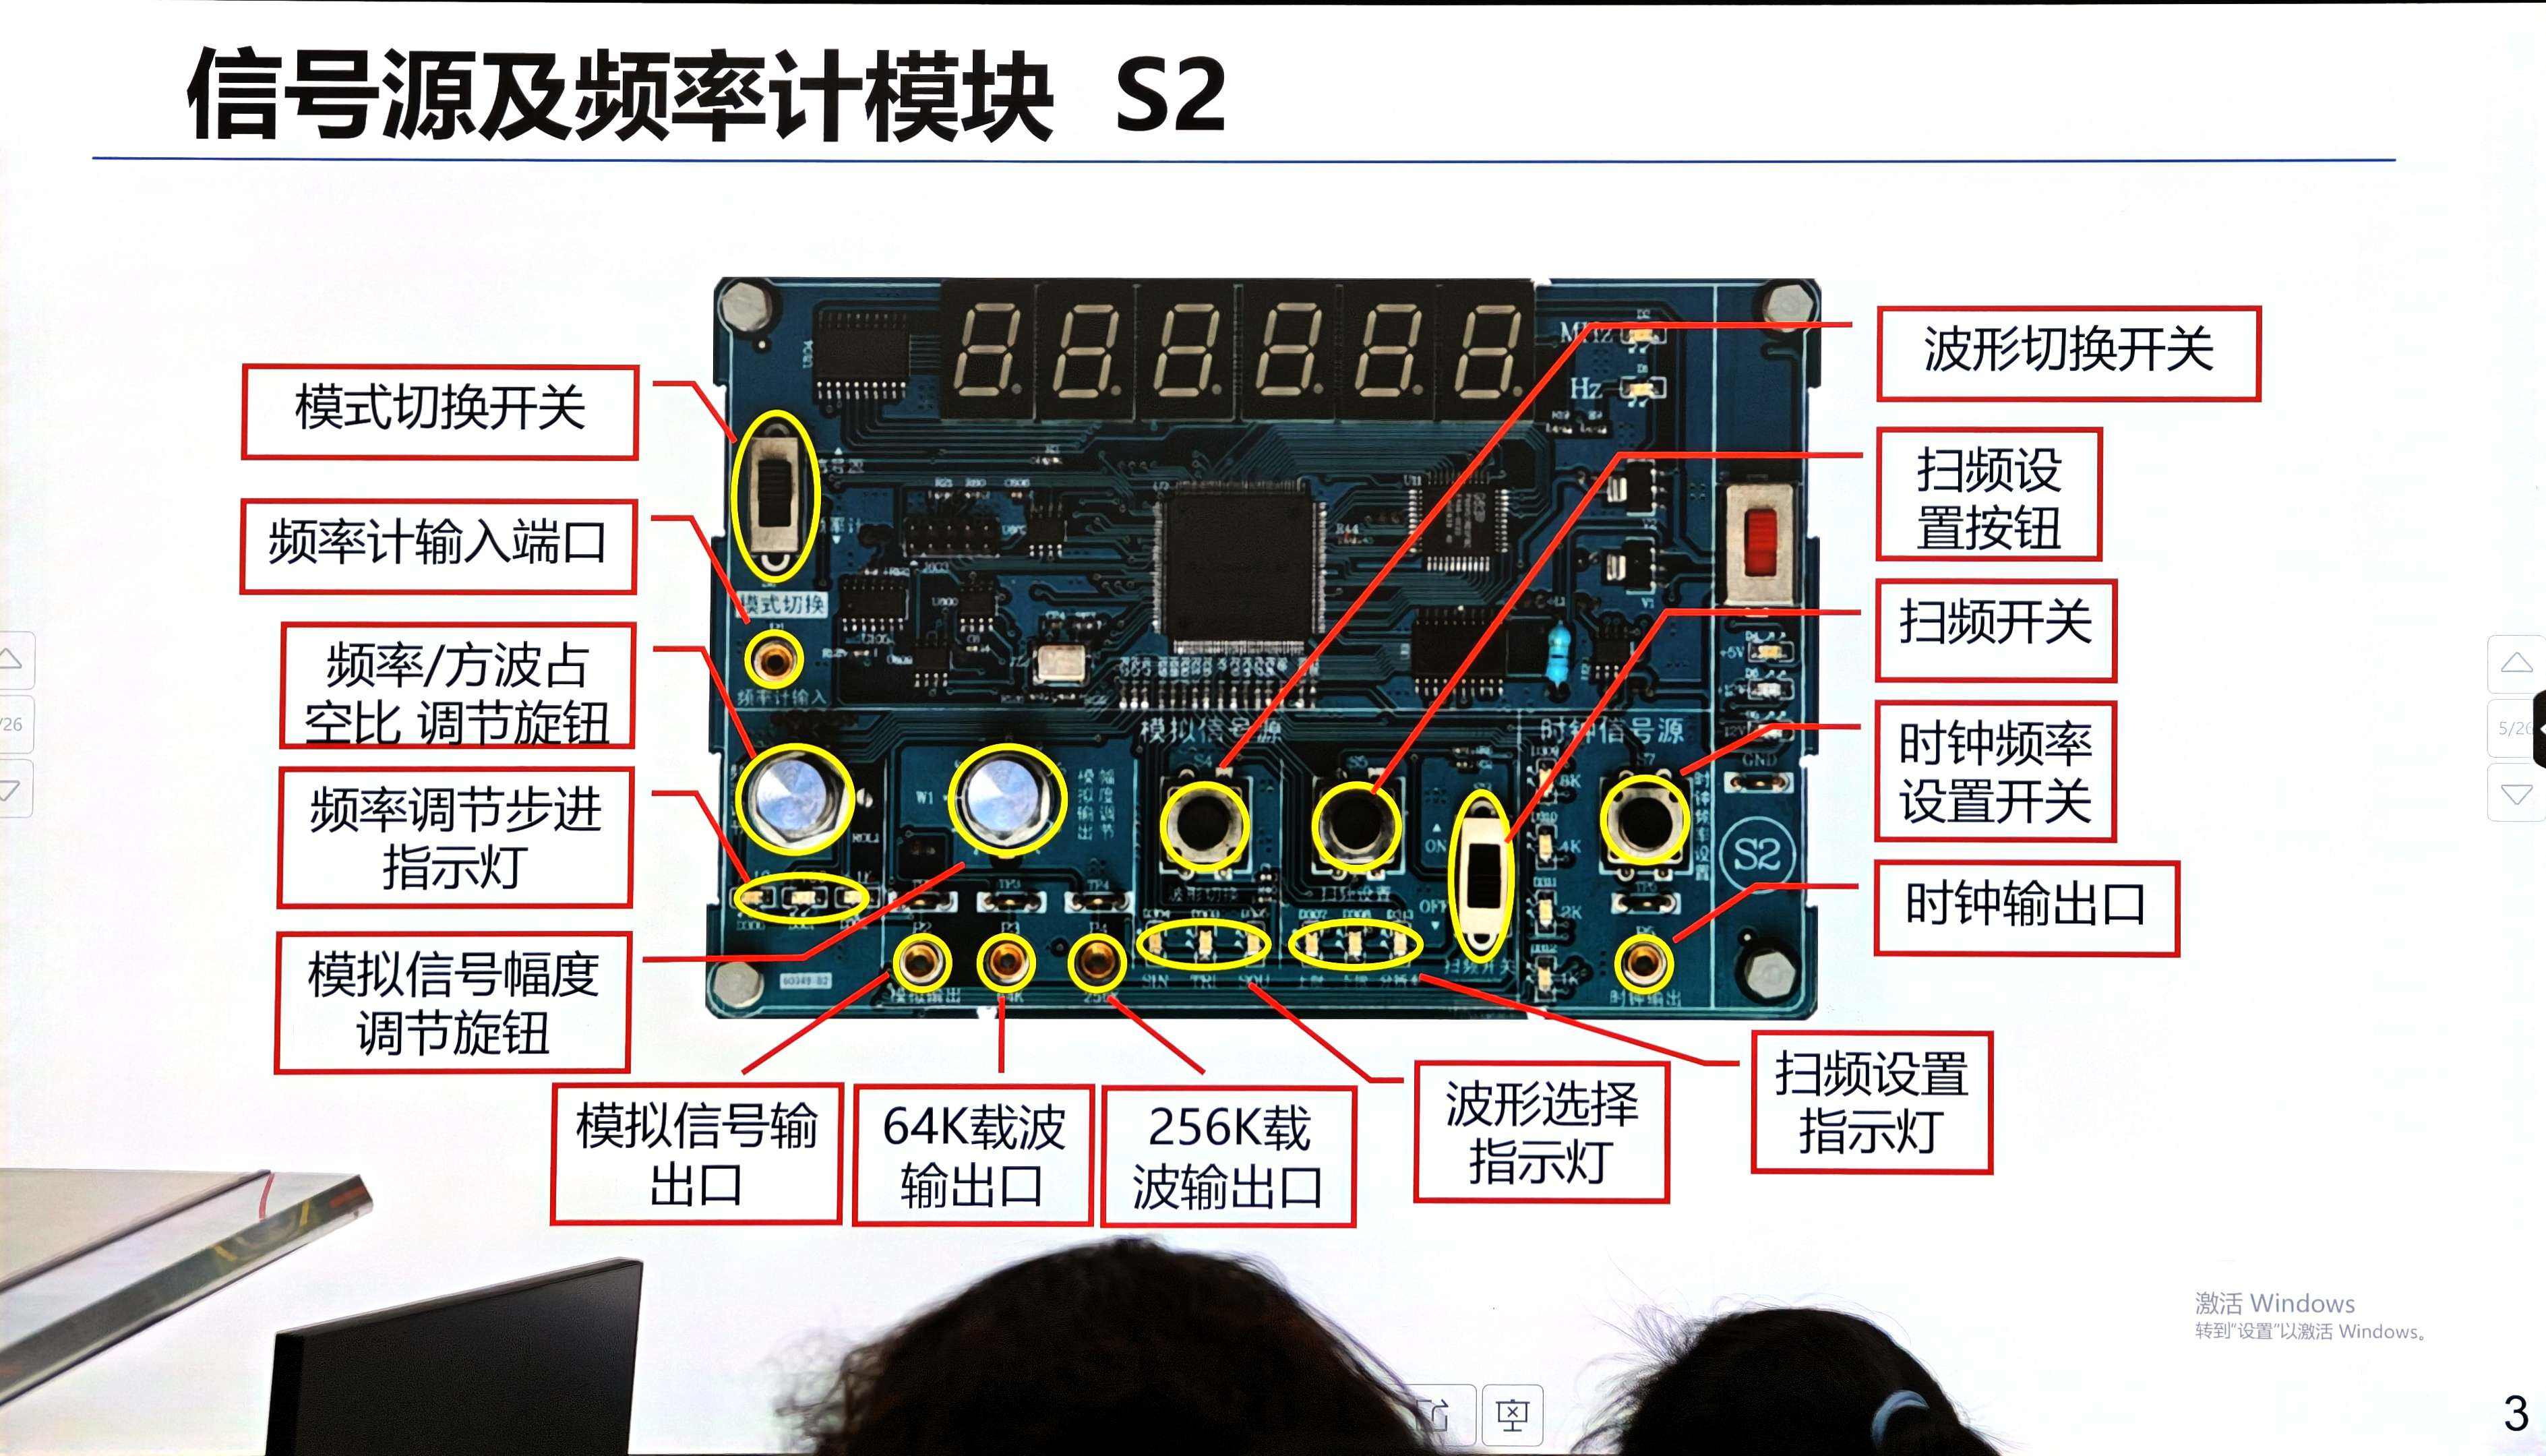
\includegraphics[width=\linewidth]{s2.jpg} % 图片宽度充满子图宽度
        \caption{信号源及频率计模块 S2}
        \label{fig:s2_sub}
    \end{subfigure}
    \hfill % 在两个子图之间添加弹性空白，使其左右散开
    % 第二个子图
    \begin{subfigure}{0.48\textwidth}
        \centering
        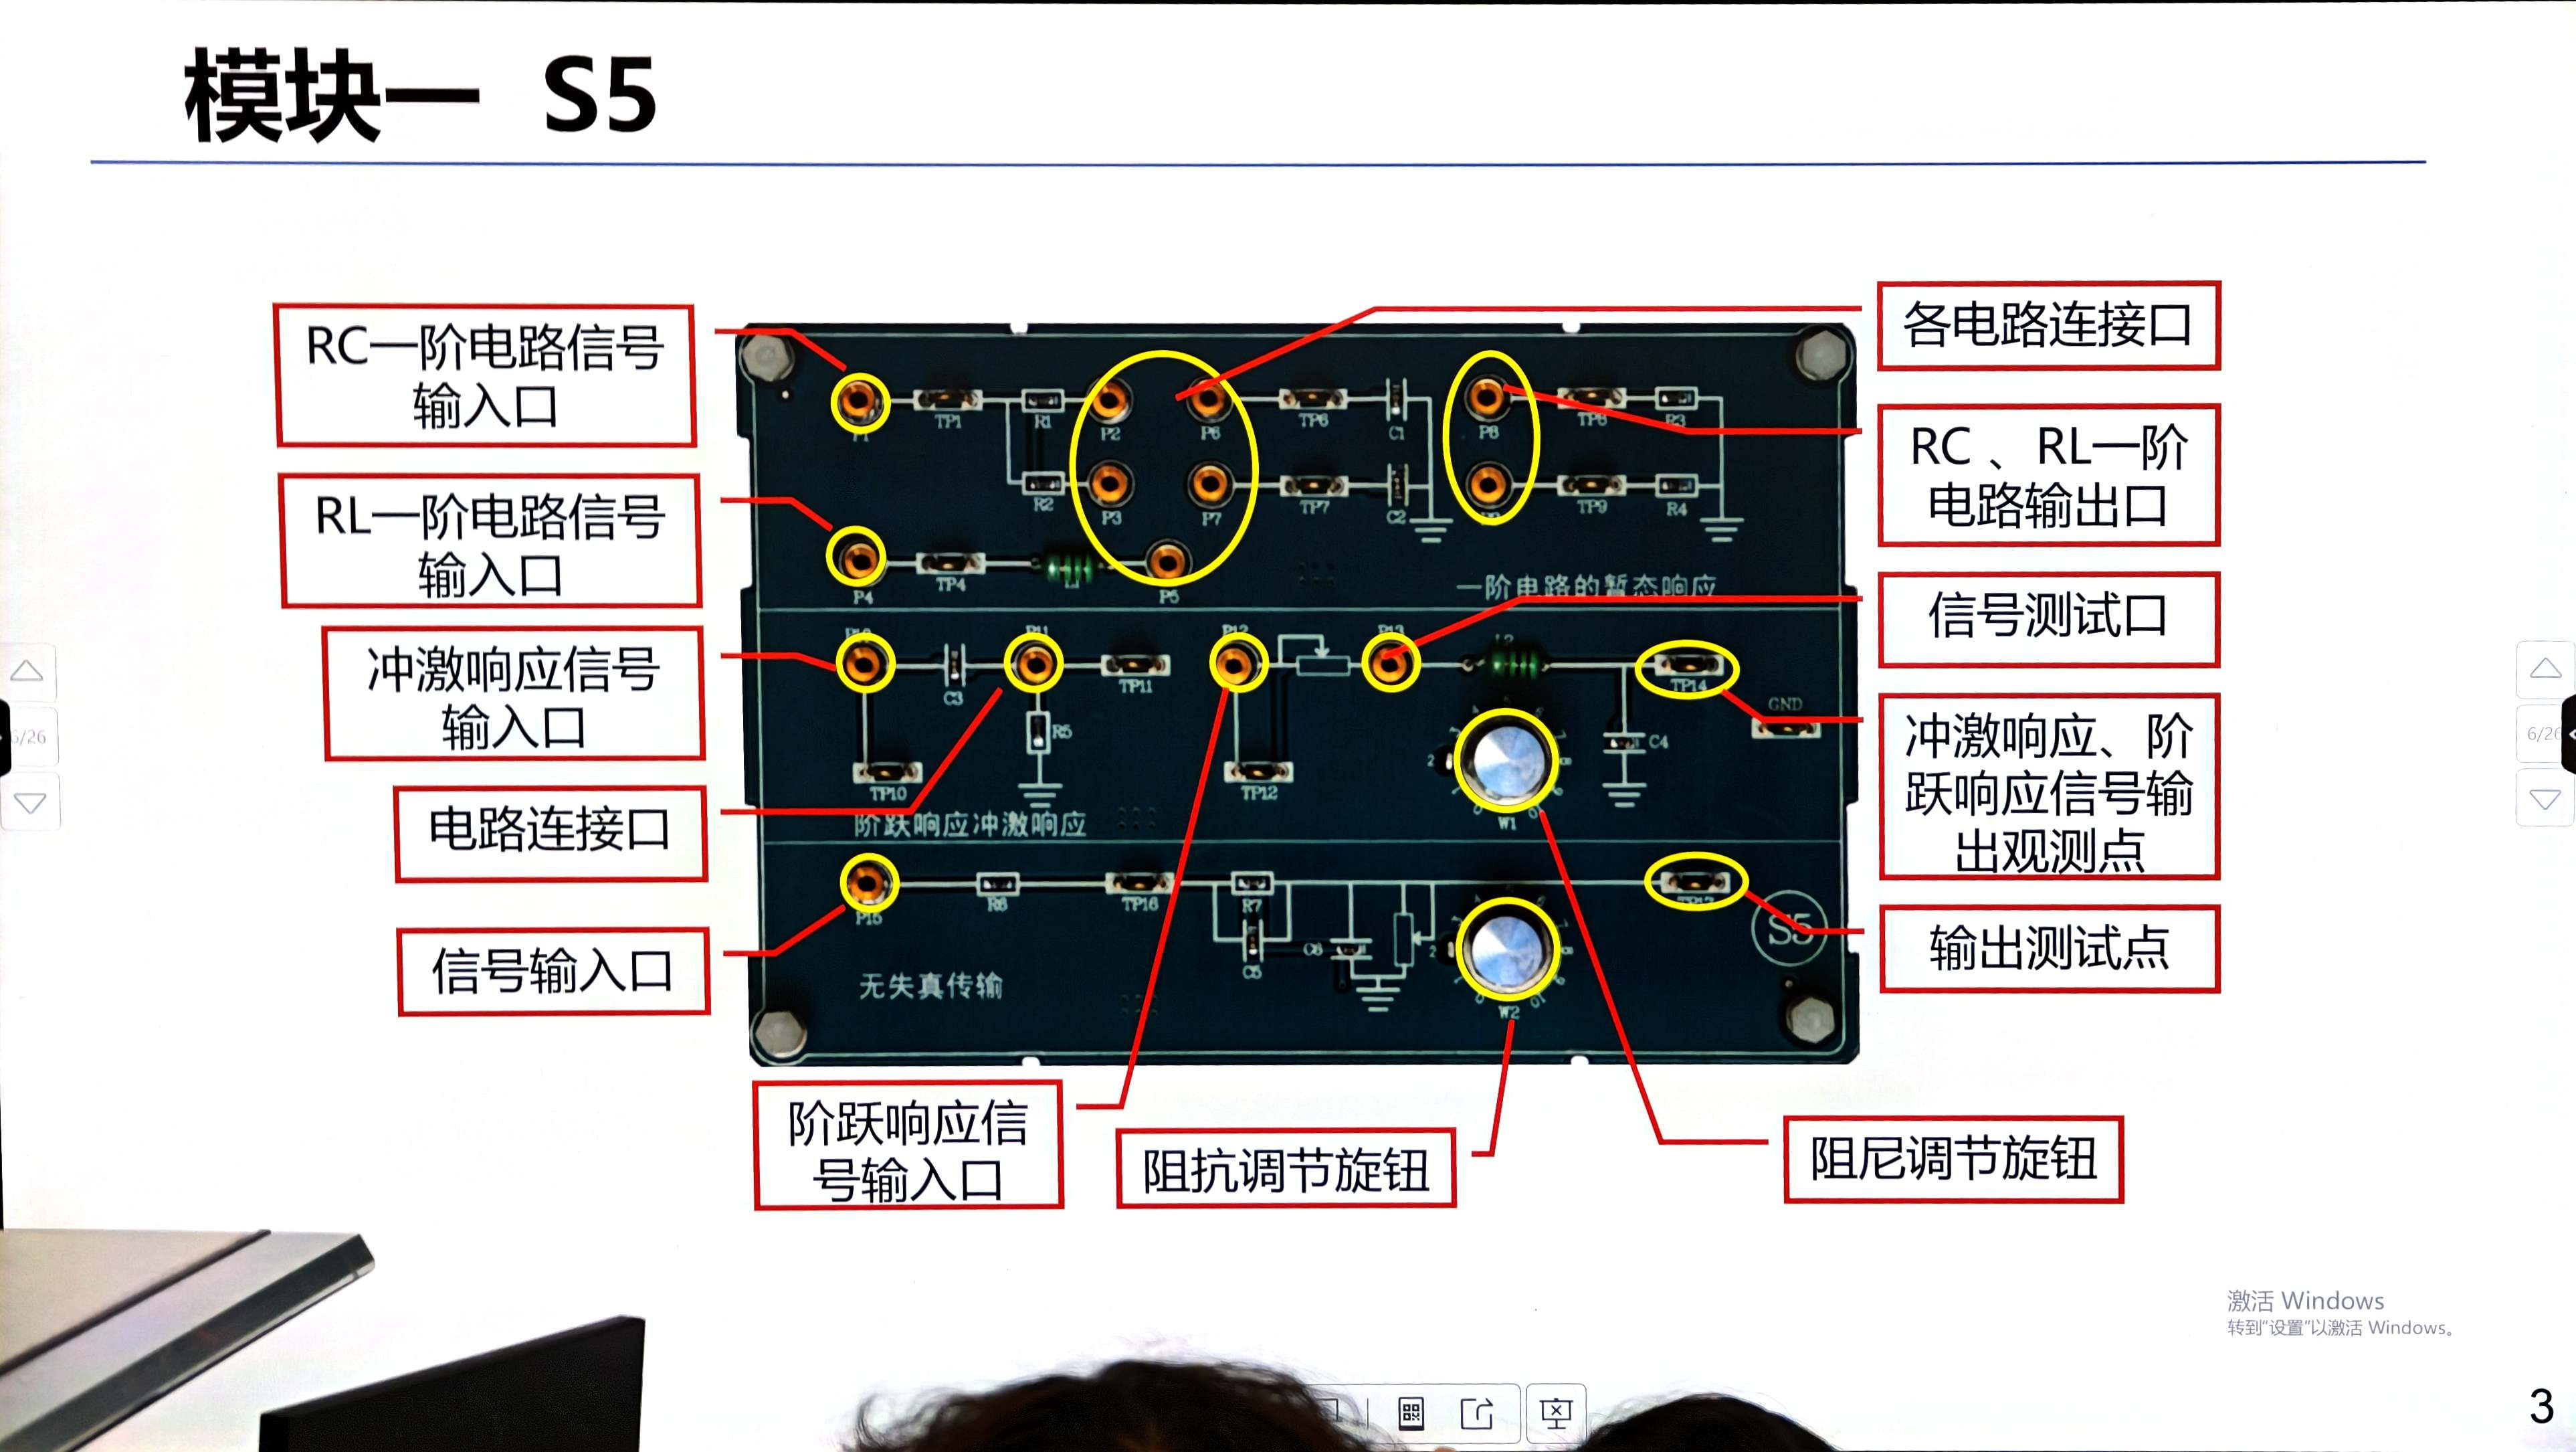
\includegraphics[width=\linewidth]{s5.jpg}
        \caption{一阶网络模块 S5}
        \label{fig:s5_sub}
    \end{subfigure}
    
    \caption{实验核心模块} % 整个图的总标题
    \label{fig:modules}
\end{figure}

\section{实验原理}

\subsection{基本概念}
对于一个线性时不变（LTI）系统，其动态特性可以通过系统对特定输入信号的响应来描述。其中，最基本的两种响应是单位冲激响应和单位阶跃响应。

\begin{itemize}
    \item \textbf{单位冲激响应}: 当输入信号为单位冲激函数 $\delta(t)$ 时，系统产生的零状态响应称为单位冲激响应，记为 $h(t)$。如图 \ref{fig:impulse_response} 所示。
    \item \textbf{单位阶跃响应}: 当输入信号为单位阶跃函数 $u(t)$ 时，系统产生的零状态响应称为单位阶跃响应，记为 $g(t)$。如图 \ref{fig:step_response} 所示。
\end{itemize}

冲激响应与阶跃响应之间存在密切的微积分关系：阶跃响应是冲激响应的积分，而冲激响应是阶跃响应的导数。
\[ g(t) = \int_{0}^{t} h(\tau) d\tau \quad \Leftrightarrow \quad h(t) = \frac{d g(t)}{dt} \]

\begin{figure}[htbp]
    \centering
    \begin{subfigure}{0.48\textwidth}
        \centering
        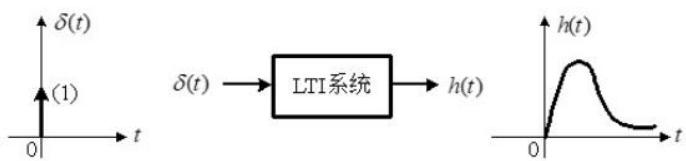
\includegraphics[width=\linewidth]{fig_impulse_response.png}
        \caption{冲激响应示意图}
        \label{fig:impulse_response}
    \end{subfigure}
    \hfill
    \begin{subfigure}{0.48\textwidth}
        \centering
        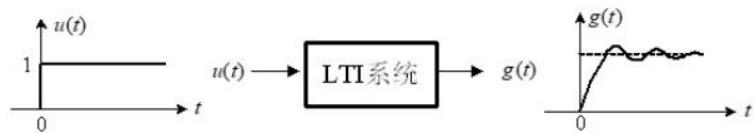
\includegraphics[width=\linewidth]{fig_step_response.png}
        \caption{阶跃响应示意图}
        \label{fig:step_response}
    \end{subfigure}
    \caption{LTI 系统的基本响应}
    \label{fig:lti_responses}
\end{figure}


\subsection{RLC 串联电路的响应分析}
本实验研究的对象是二阶 RLC 串联电路，其阶跃响应与冲激响应的电路连接如图 \ref{fig:rlc_circuits} 所示。根据电阻 $R$、电感 $L$ 和电容 $C$ 的取值不同，系统的响应会呈现出三种不同的状态：
\begin{enumerate}
    \item \textbf{过阻尼状态}: 当 $R > 2\sqrt{\frac{L}{C}}$ 时，响应曲线无振荡，缓慢上升至稳态值。
    \item \textbf{临界阻尼状态}: 当 $R = 2\sqrt{\frac{L}{C}}$ 时，响应以最快的速度到达稳态值且无超调。
    \item \textbf{欠阻尼状态}: 当 $R < 2\sqrt{\frac{L}{C}}$ 时，响应曲线将出现振荡和超调现象。
\end{enumerate}

\begin{figure}[htbp]
    \centering
    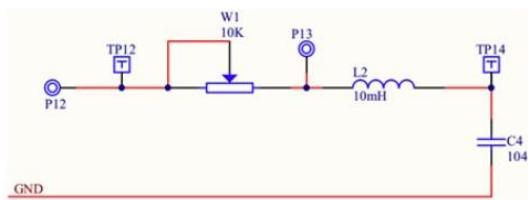
\includegraphics[width=0.4\textwidth]{fig_rlc_circuits.png}
    \caption{RLC 串联电路连接示意图}
    \label{fig:rlc_circuits}
\end{figure}


\subsection{动态性能指标}
对于欠阻尼二阶系统的阶跃响应，通常使用一系列动态性能指标来衡量其响应的快速性和稳定性，如图 \ref{fig:indicators} 所示。
\begin{description}
    \item[上升时间 ($t_r$)] 响应从稳态值的 10\% 上升到 90\% 所需的时间（或从0首次到达稳态值的时间）。
    \item[峰值时间 ($t_p$)] 响应从开始上升到第一个峰值点所需的时间。
    \item[调节时间 ($t_s$)] 响应进入并保持在稳态值的 $\pm 5\%$ (或 $\pm 2\%$) 误差带内所需的最短时间。
    \item[最大超调量 ($\delta_p$)] 响应的最大峰值 $y_{\max}$ 超出其稳态值 $y(\infty)$ 的百分比，计算公式为：
    \[ \delta_p = \frac{y_{\max} - y(\infty)}{y(\infty)} \times 100\% \]
\end{description}

\begin{figure}[htbp]
    \centering
    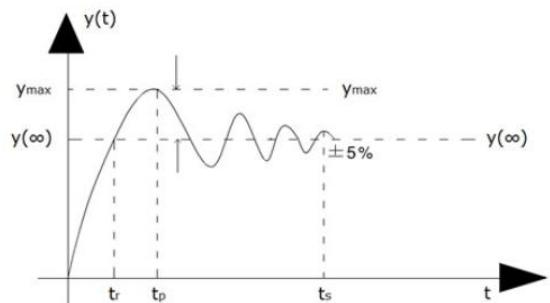
\includegraphics[width=0.4\textwidth]{fig_indicators.png}
    \caption{欠阻尼响应动态性能指标示意图}
    \label{fig:indicators}
\end{figure}

\section{实验数据与分析}

\subsection{波形观察与记录}
实验中，通过示波器观察并记录了阶跃响应和冲激响应在不同阻尼状态下的输入与输出波形，具体如下图所示。

% --- 阶跃响应波形图 ---
\begin{figure}[htbp]
    \centering
    \begin{subfigure}{0.32\textwidth}
        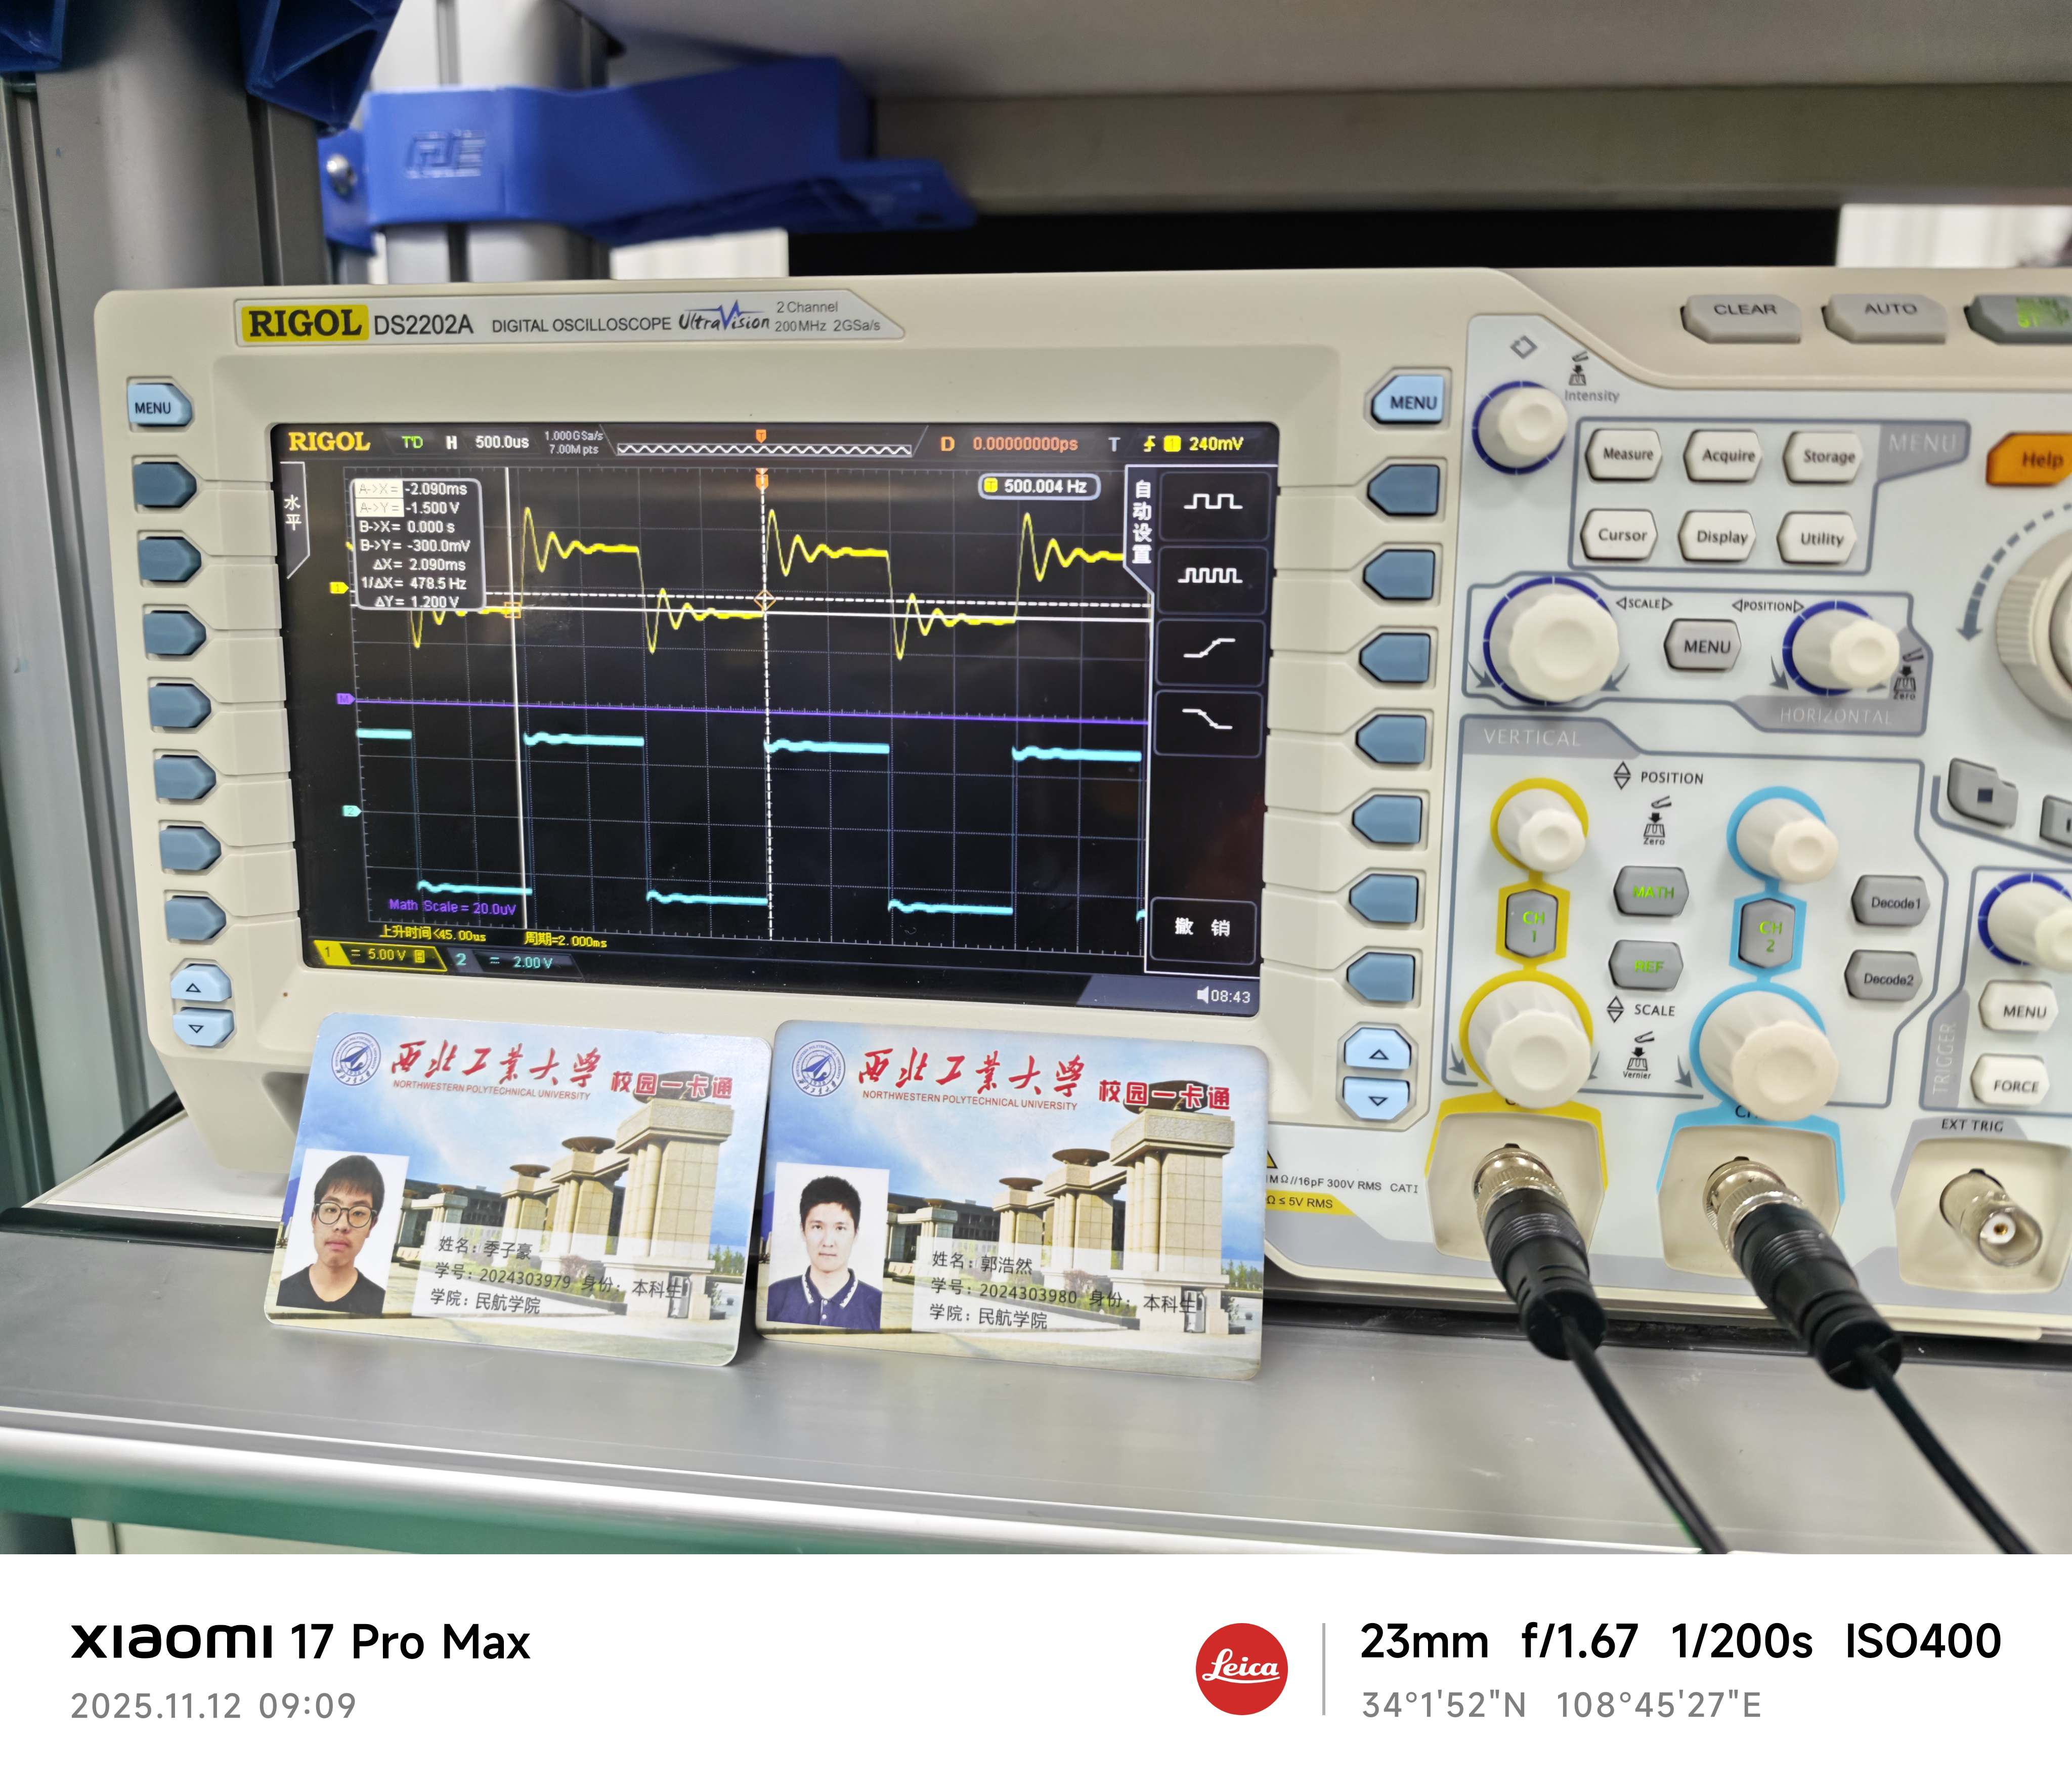
\includegraphics[width=\linewidth]{step_underdamped.jpg}
        \caption{欠阻尼状态}
        \label{fig:step_under}
    \end{subfigure}
    \hfill
    \begin{subfigure}{0.32\textwidth}
        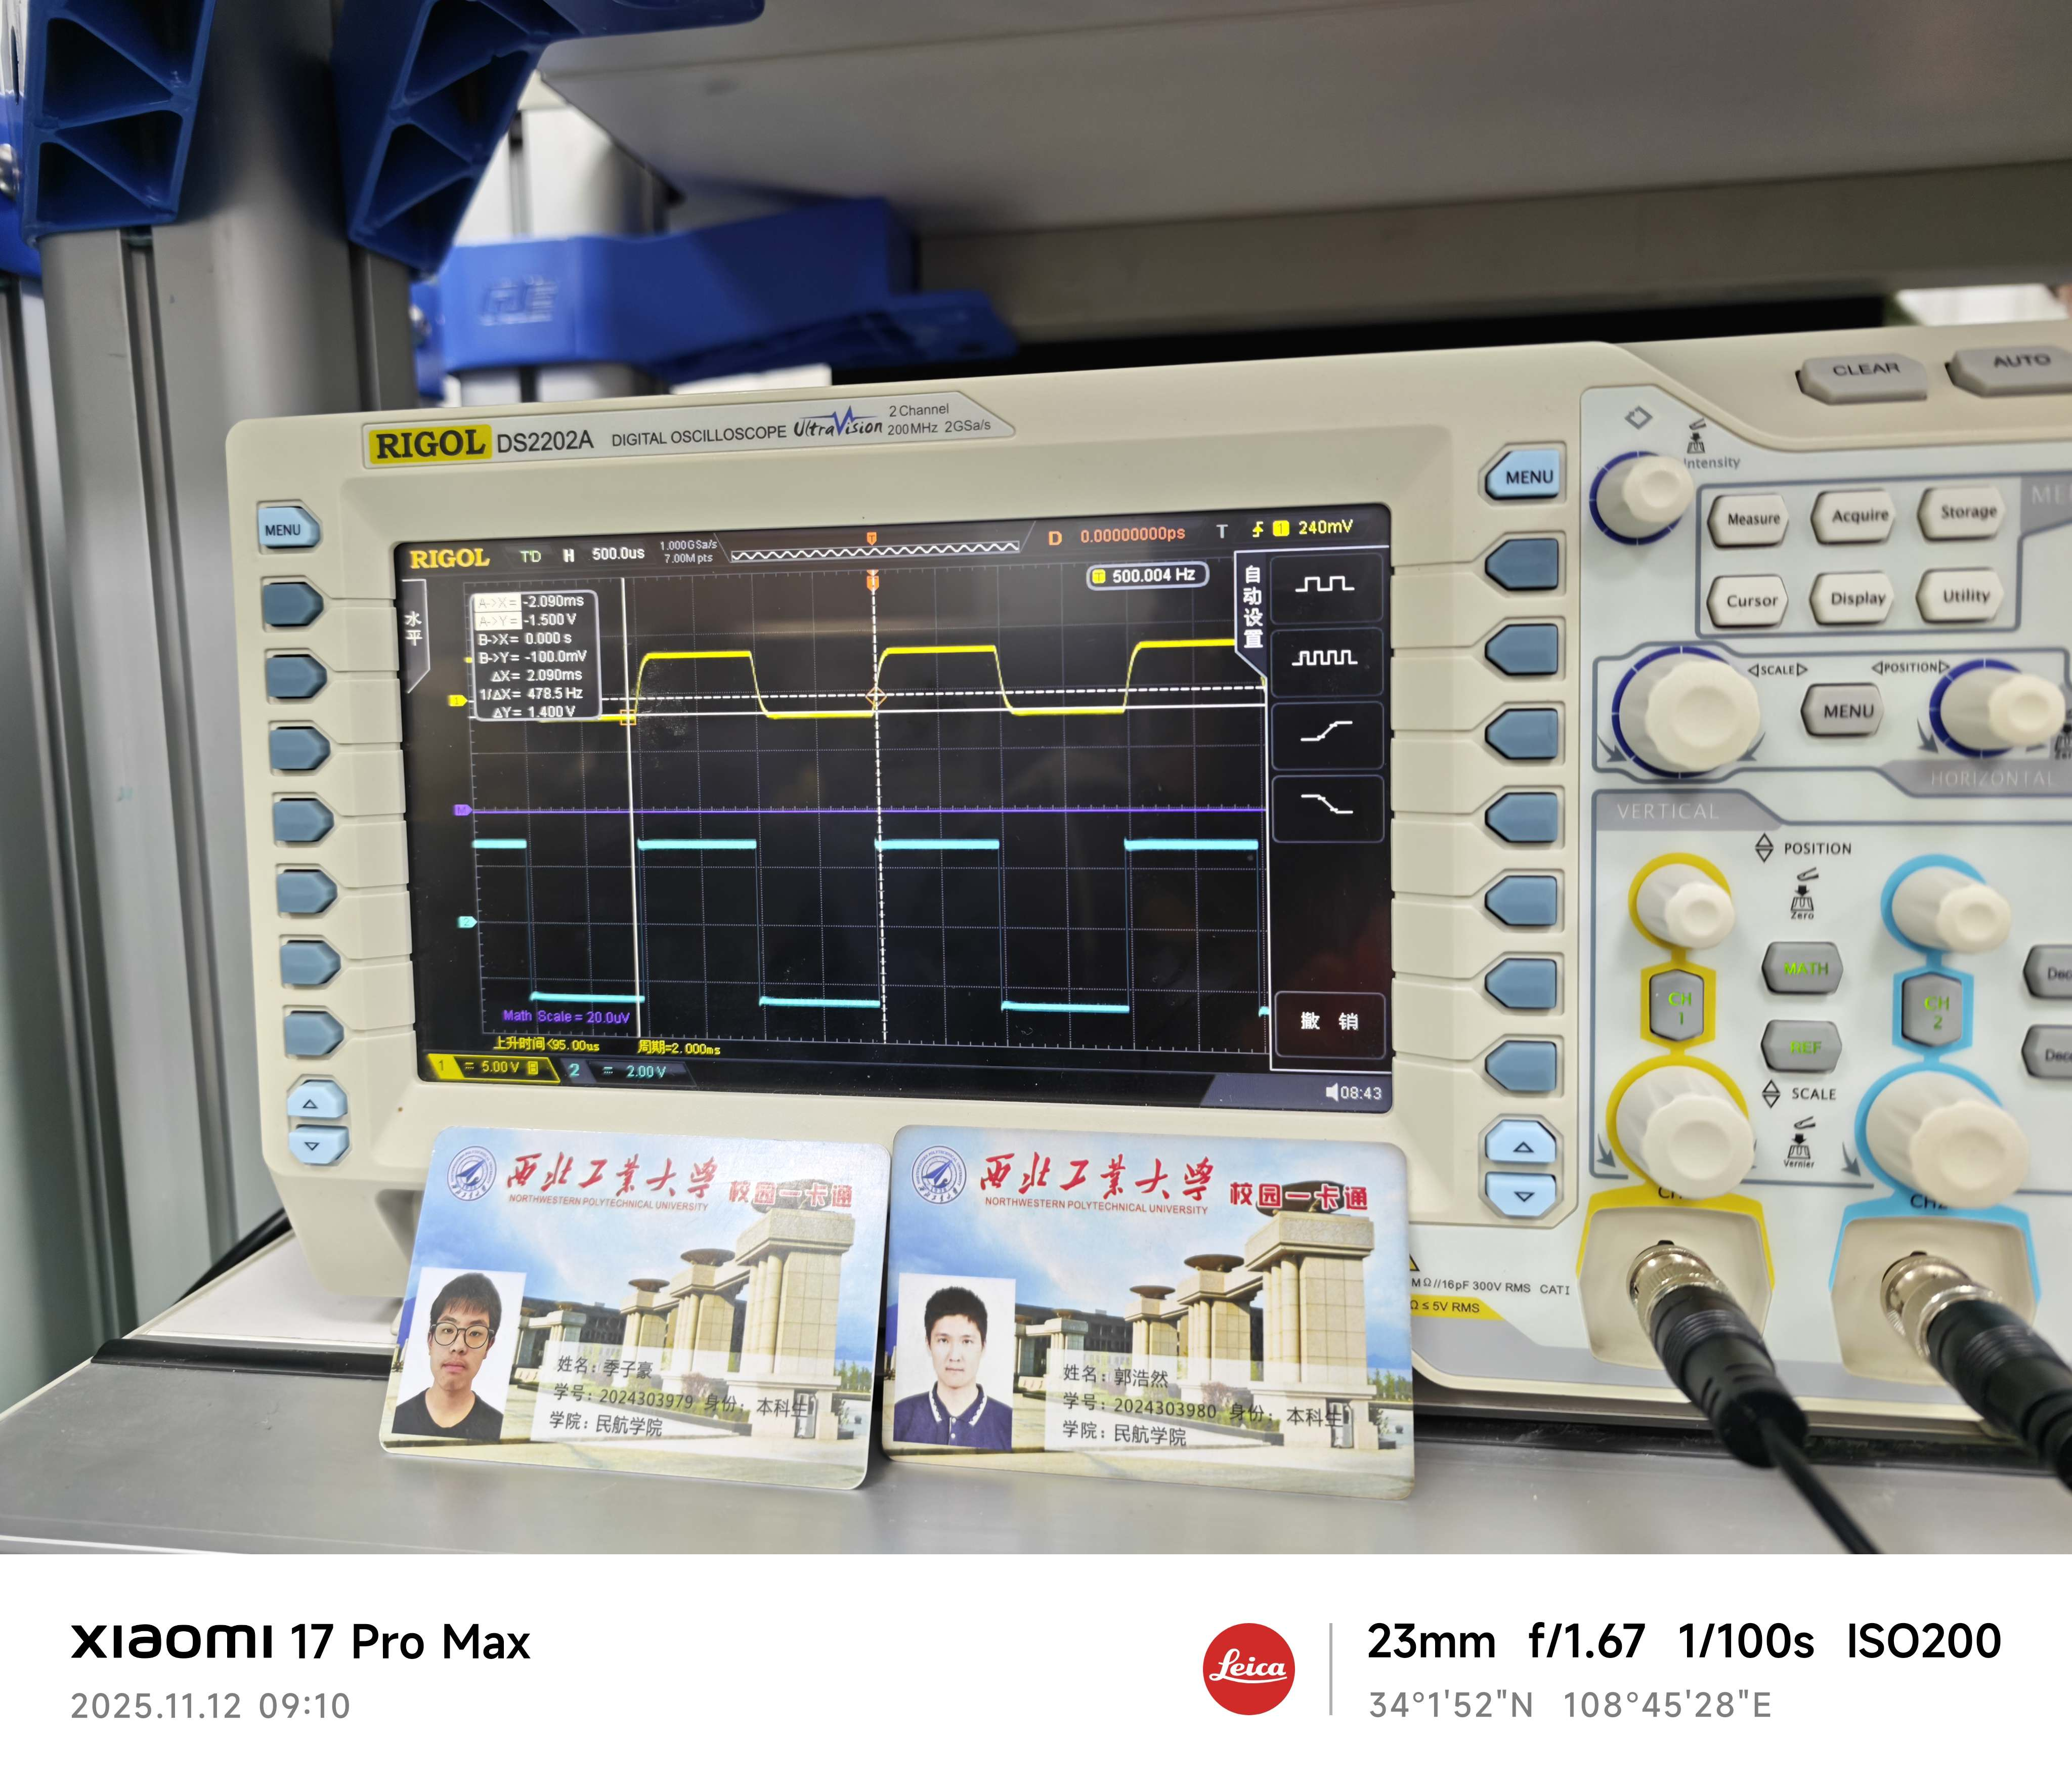
\includegraphics[width=\linewidth]{step_critical.jpg}
        \caption{临界阻尼状态}
        \label{fig:step_critical}
    \end{subfigure}
    \hfill
    \begin{subfigure}{0.32\textwidth}
        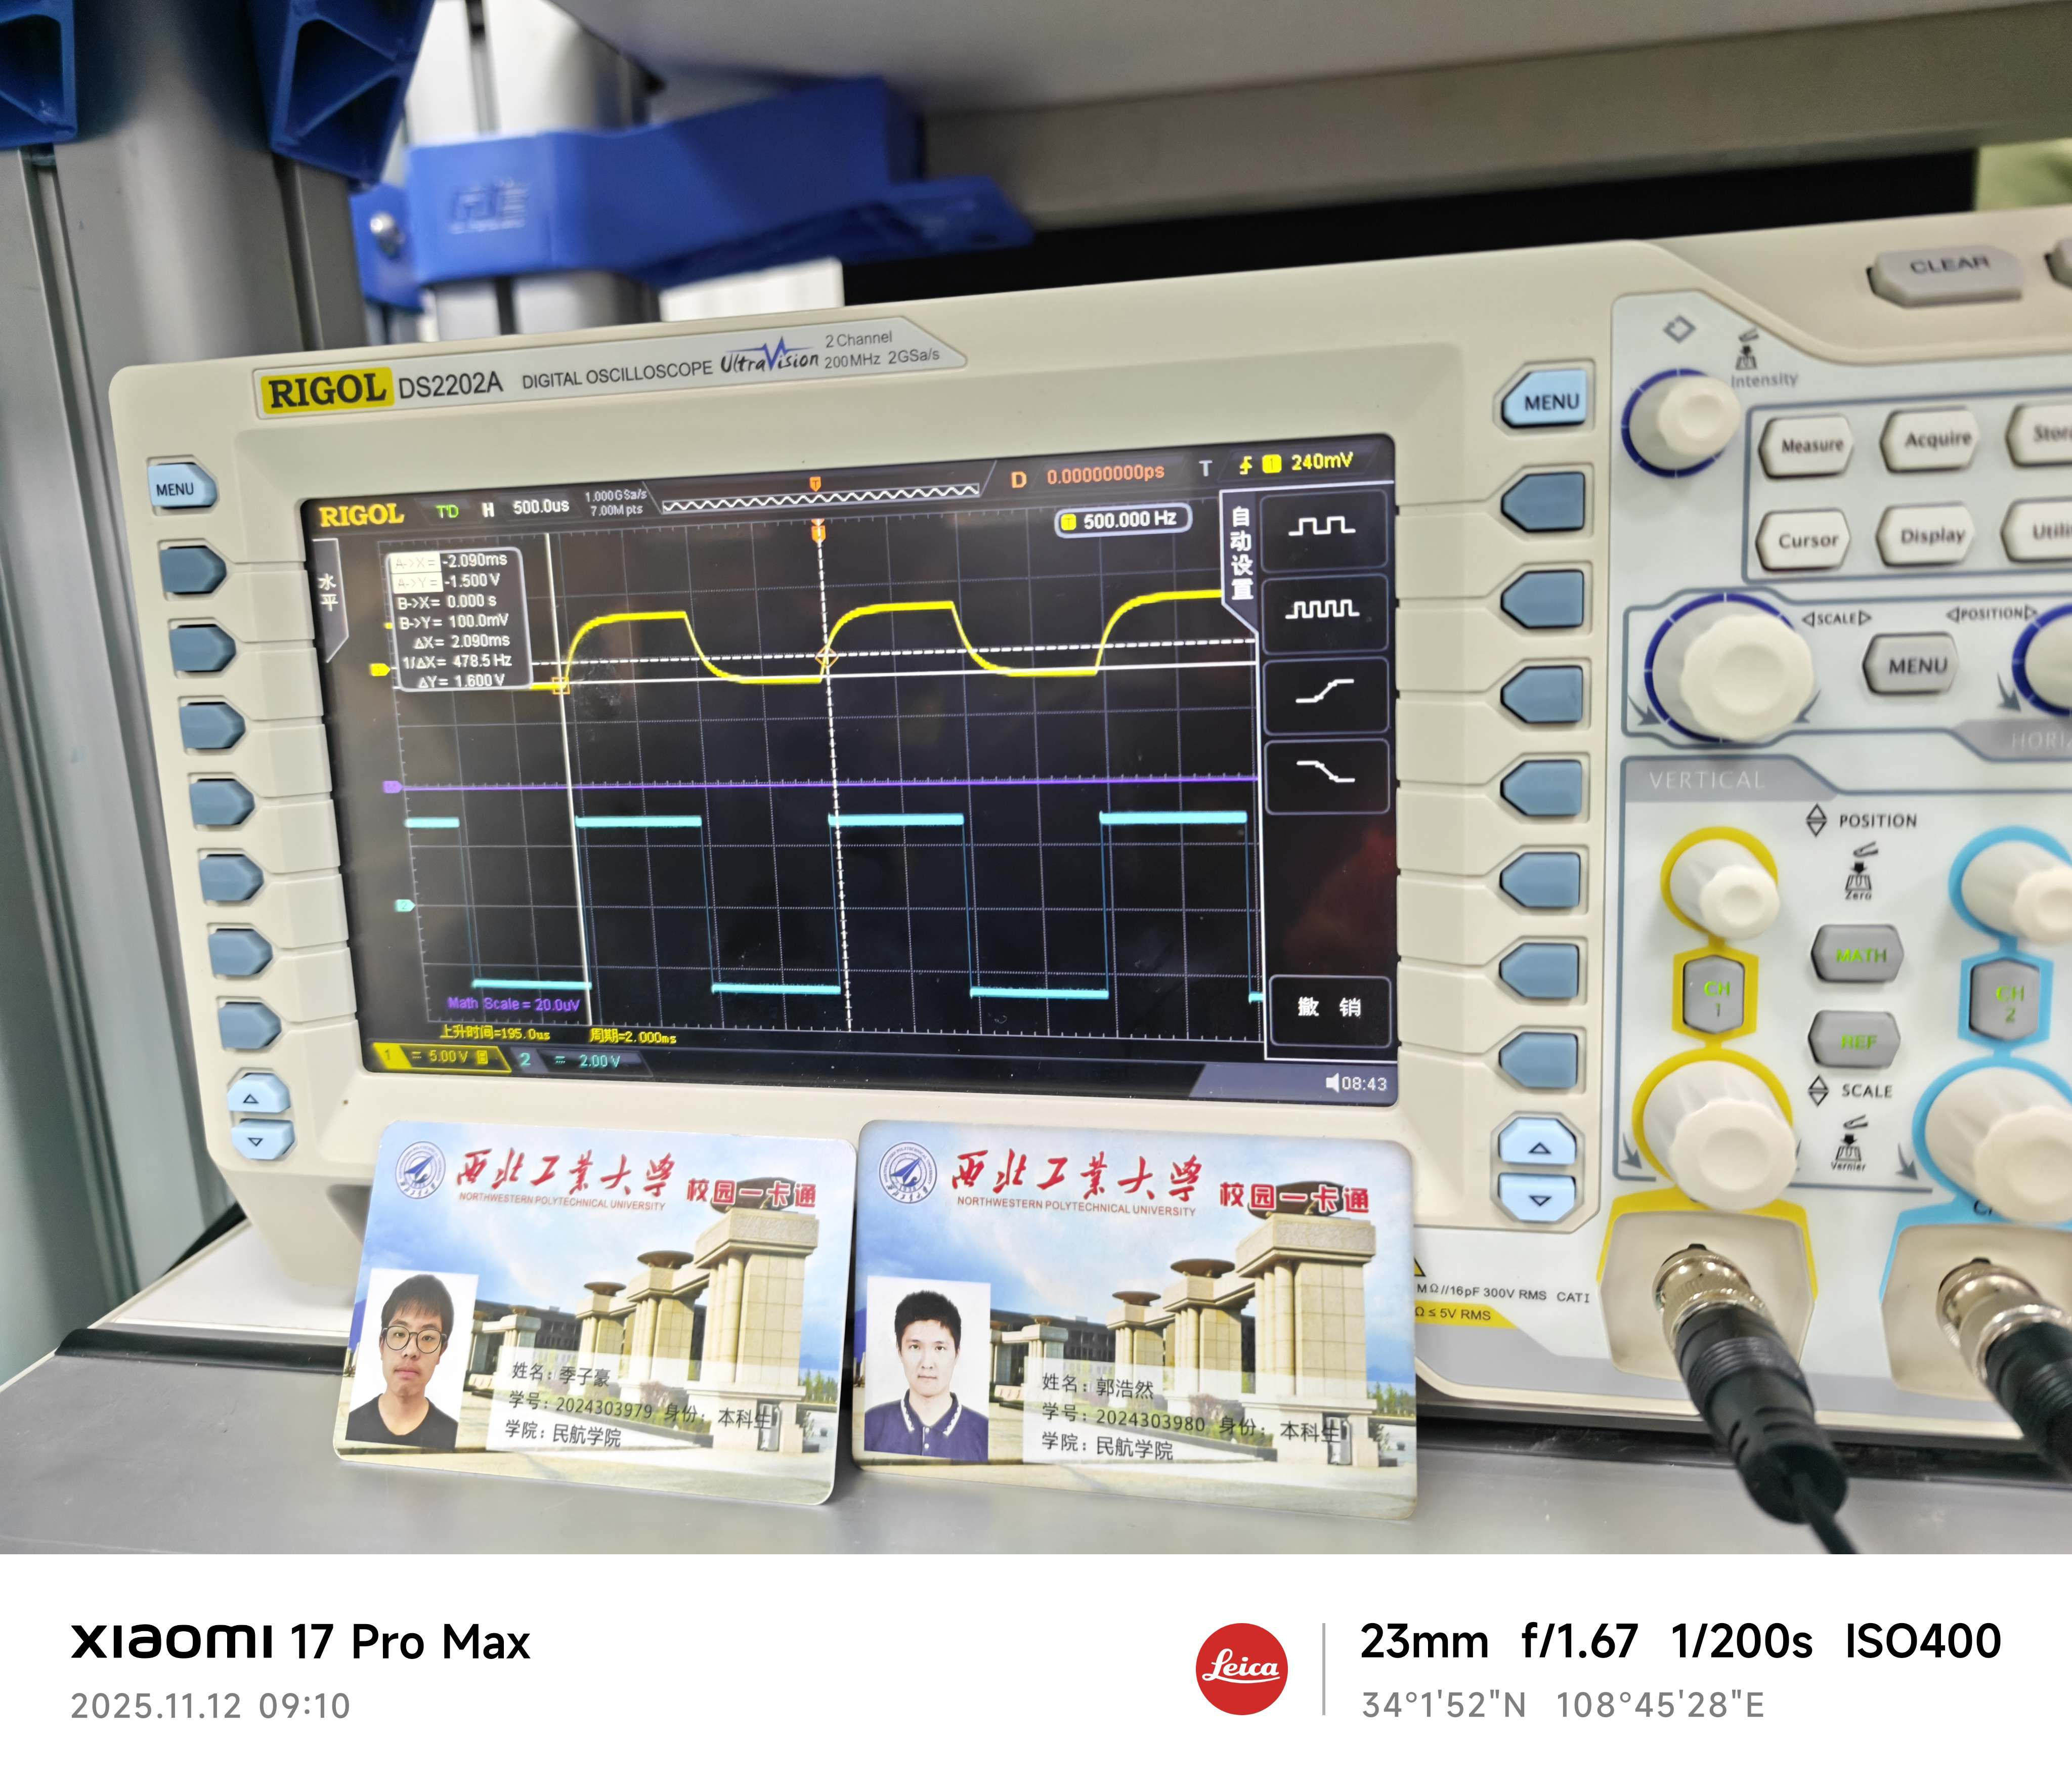
\includegraphics[width=\linewidth]{step_overdamped.jpg}
        \caption{过阻尼状态}
        \label{fig:step_over}
    \end{subfigure}
    \caption{阶跃响应在不同阻尼状态下的示波器波形}
    \label{fig:step_waveforms}
\end{figure}

% --- 冲激响应波形图 ---
\begin{figure}[htbp]
    \centering
    \begin{subfigure}{0.32\textwidth}
        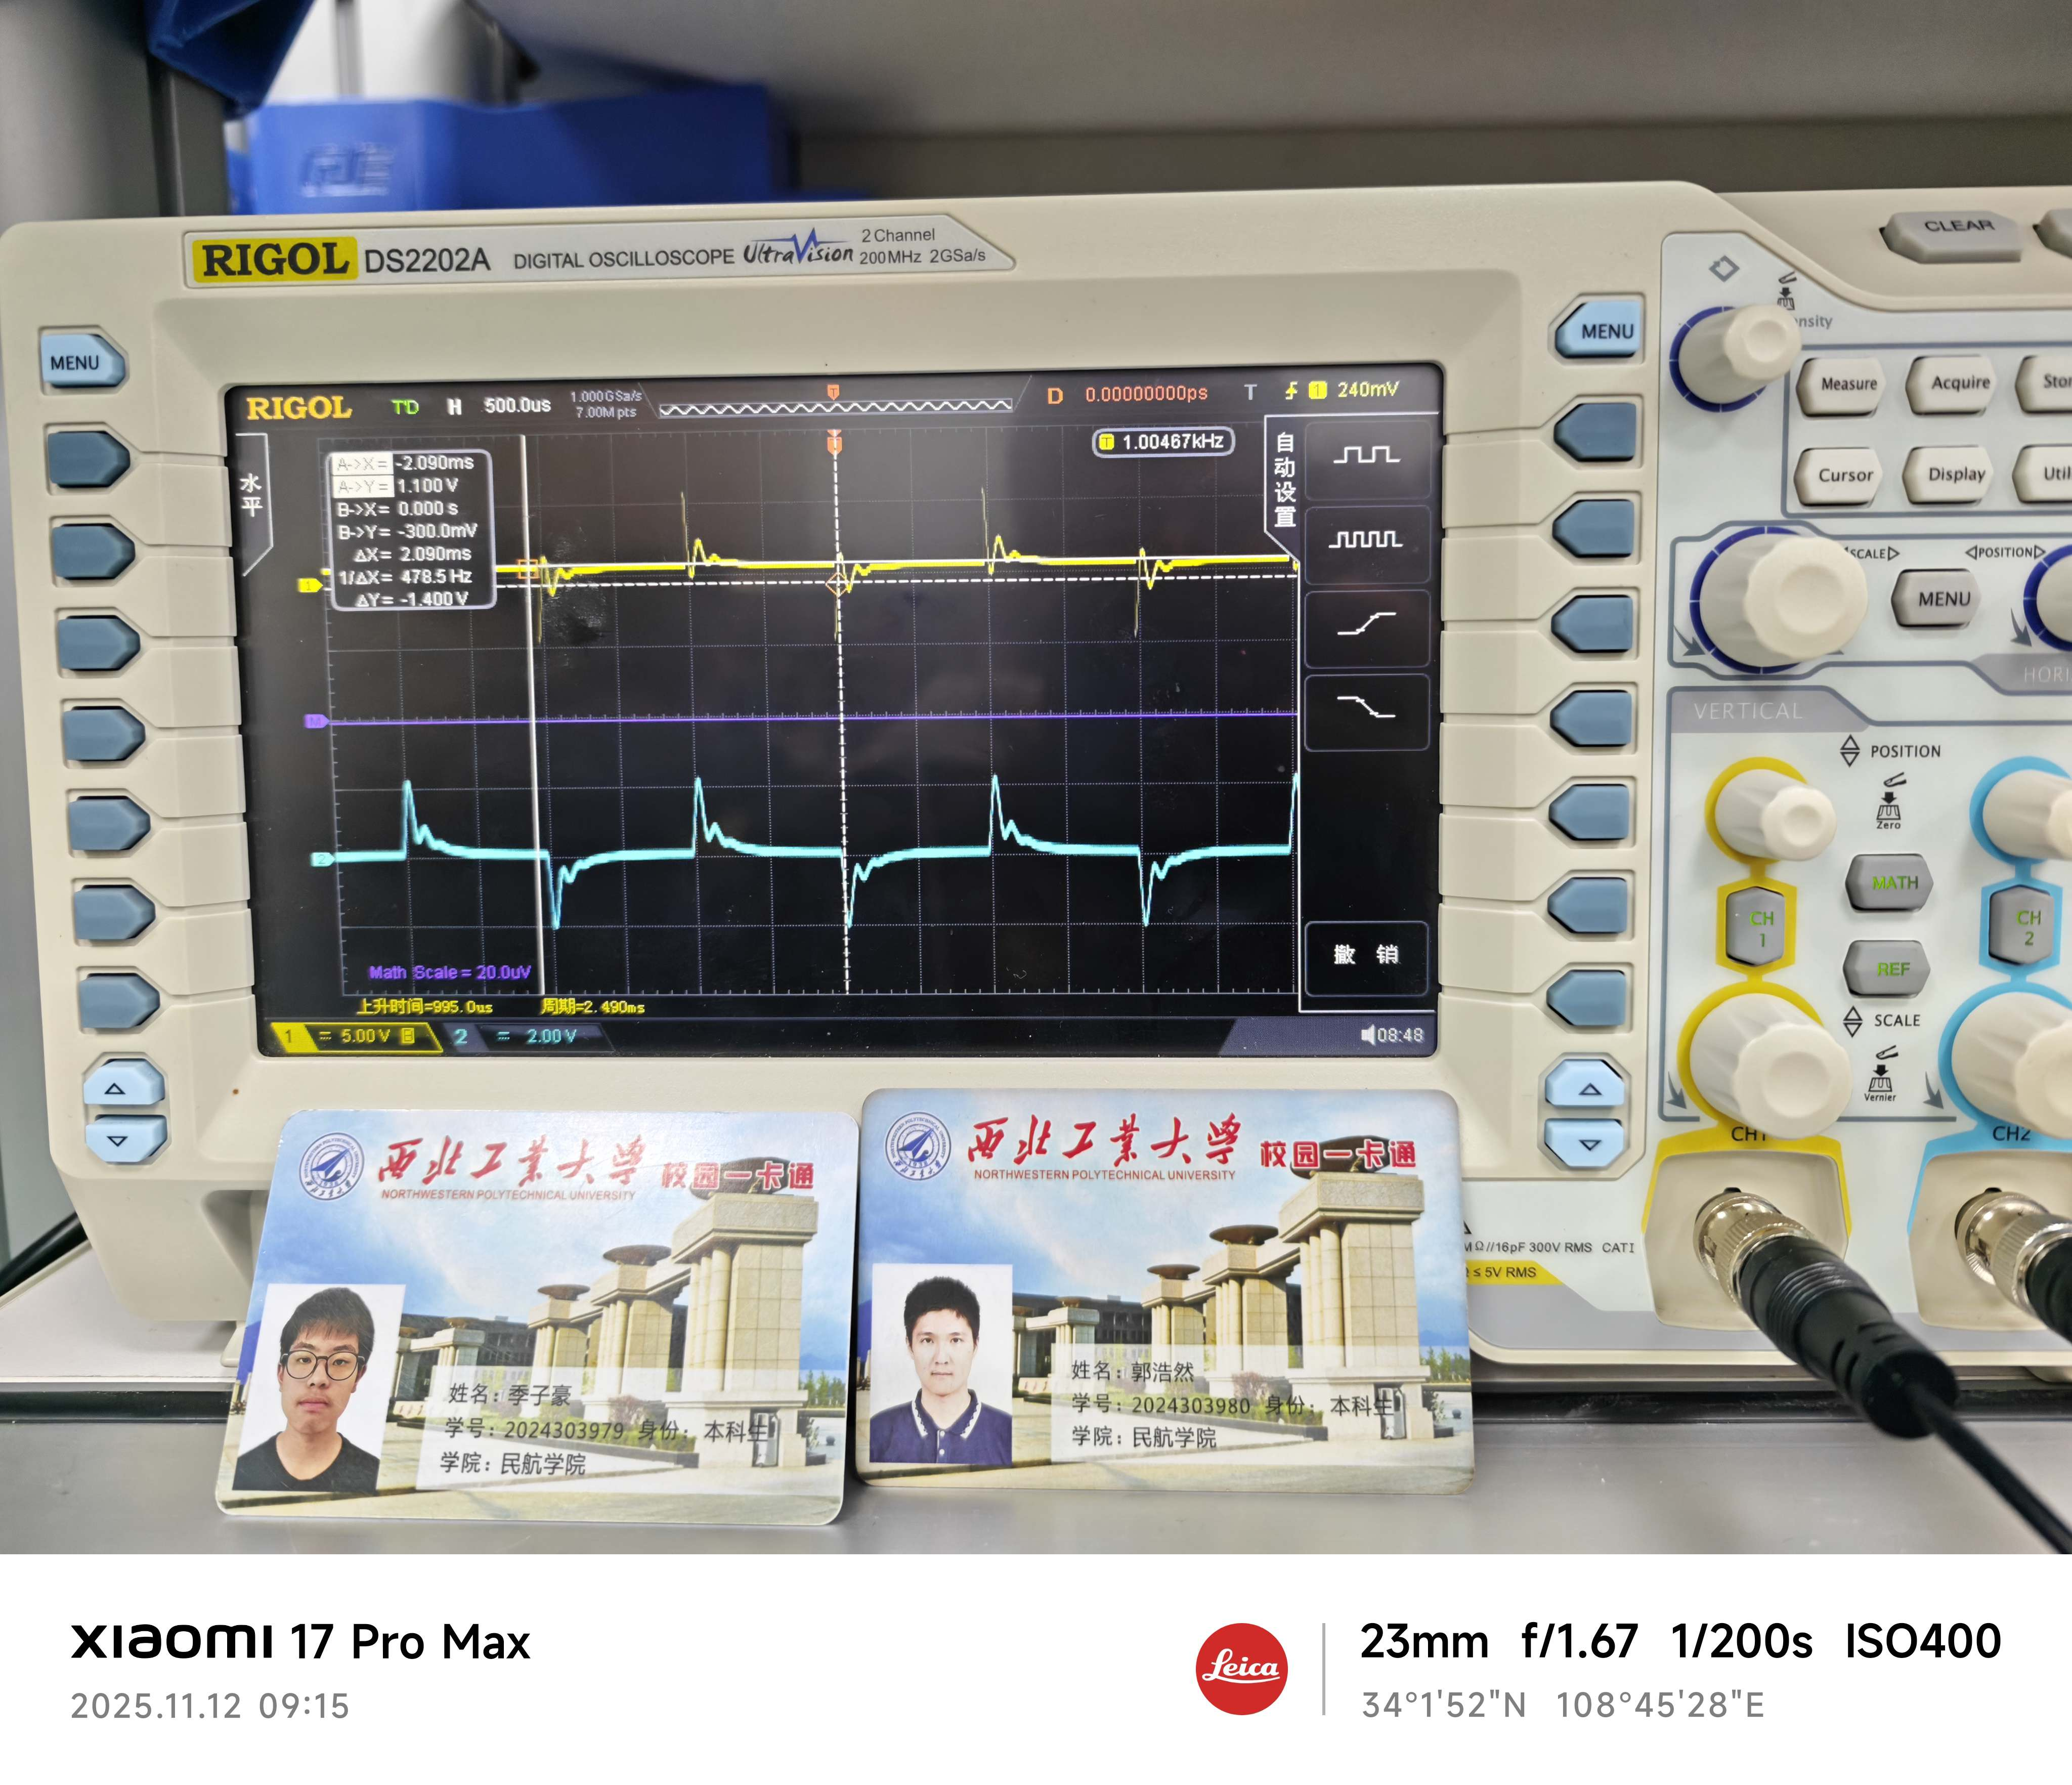
\includegraphics[width=\linewidth]{impulse_underdamped.jpg}
        \caption{欠阻尼状态}
        \label{fig:impulse_under}
    \end{subfigure}
    \hfill
    \begin{subfigure}{0.32\textwidth}
        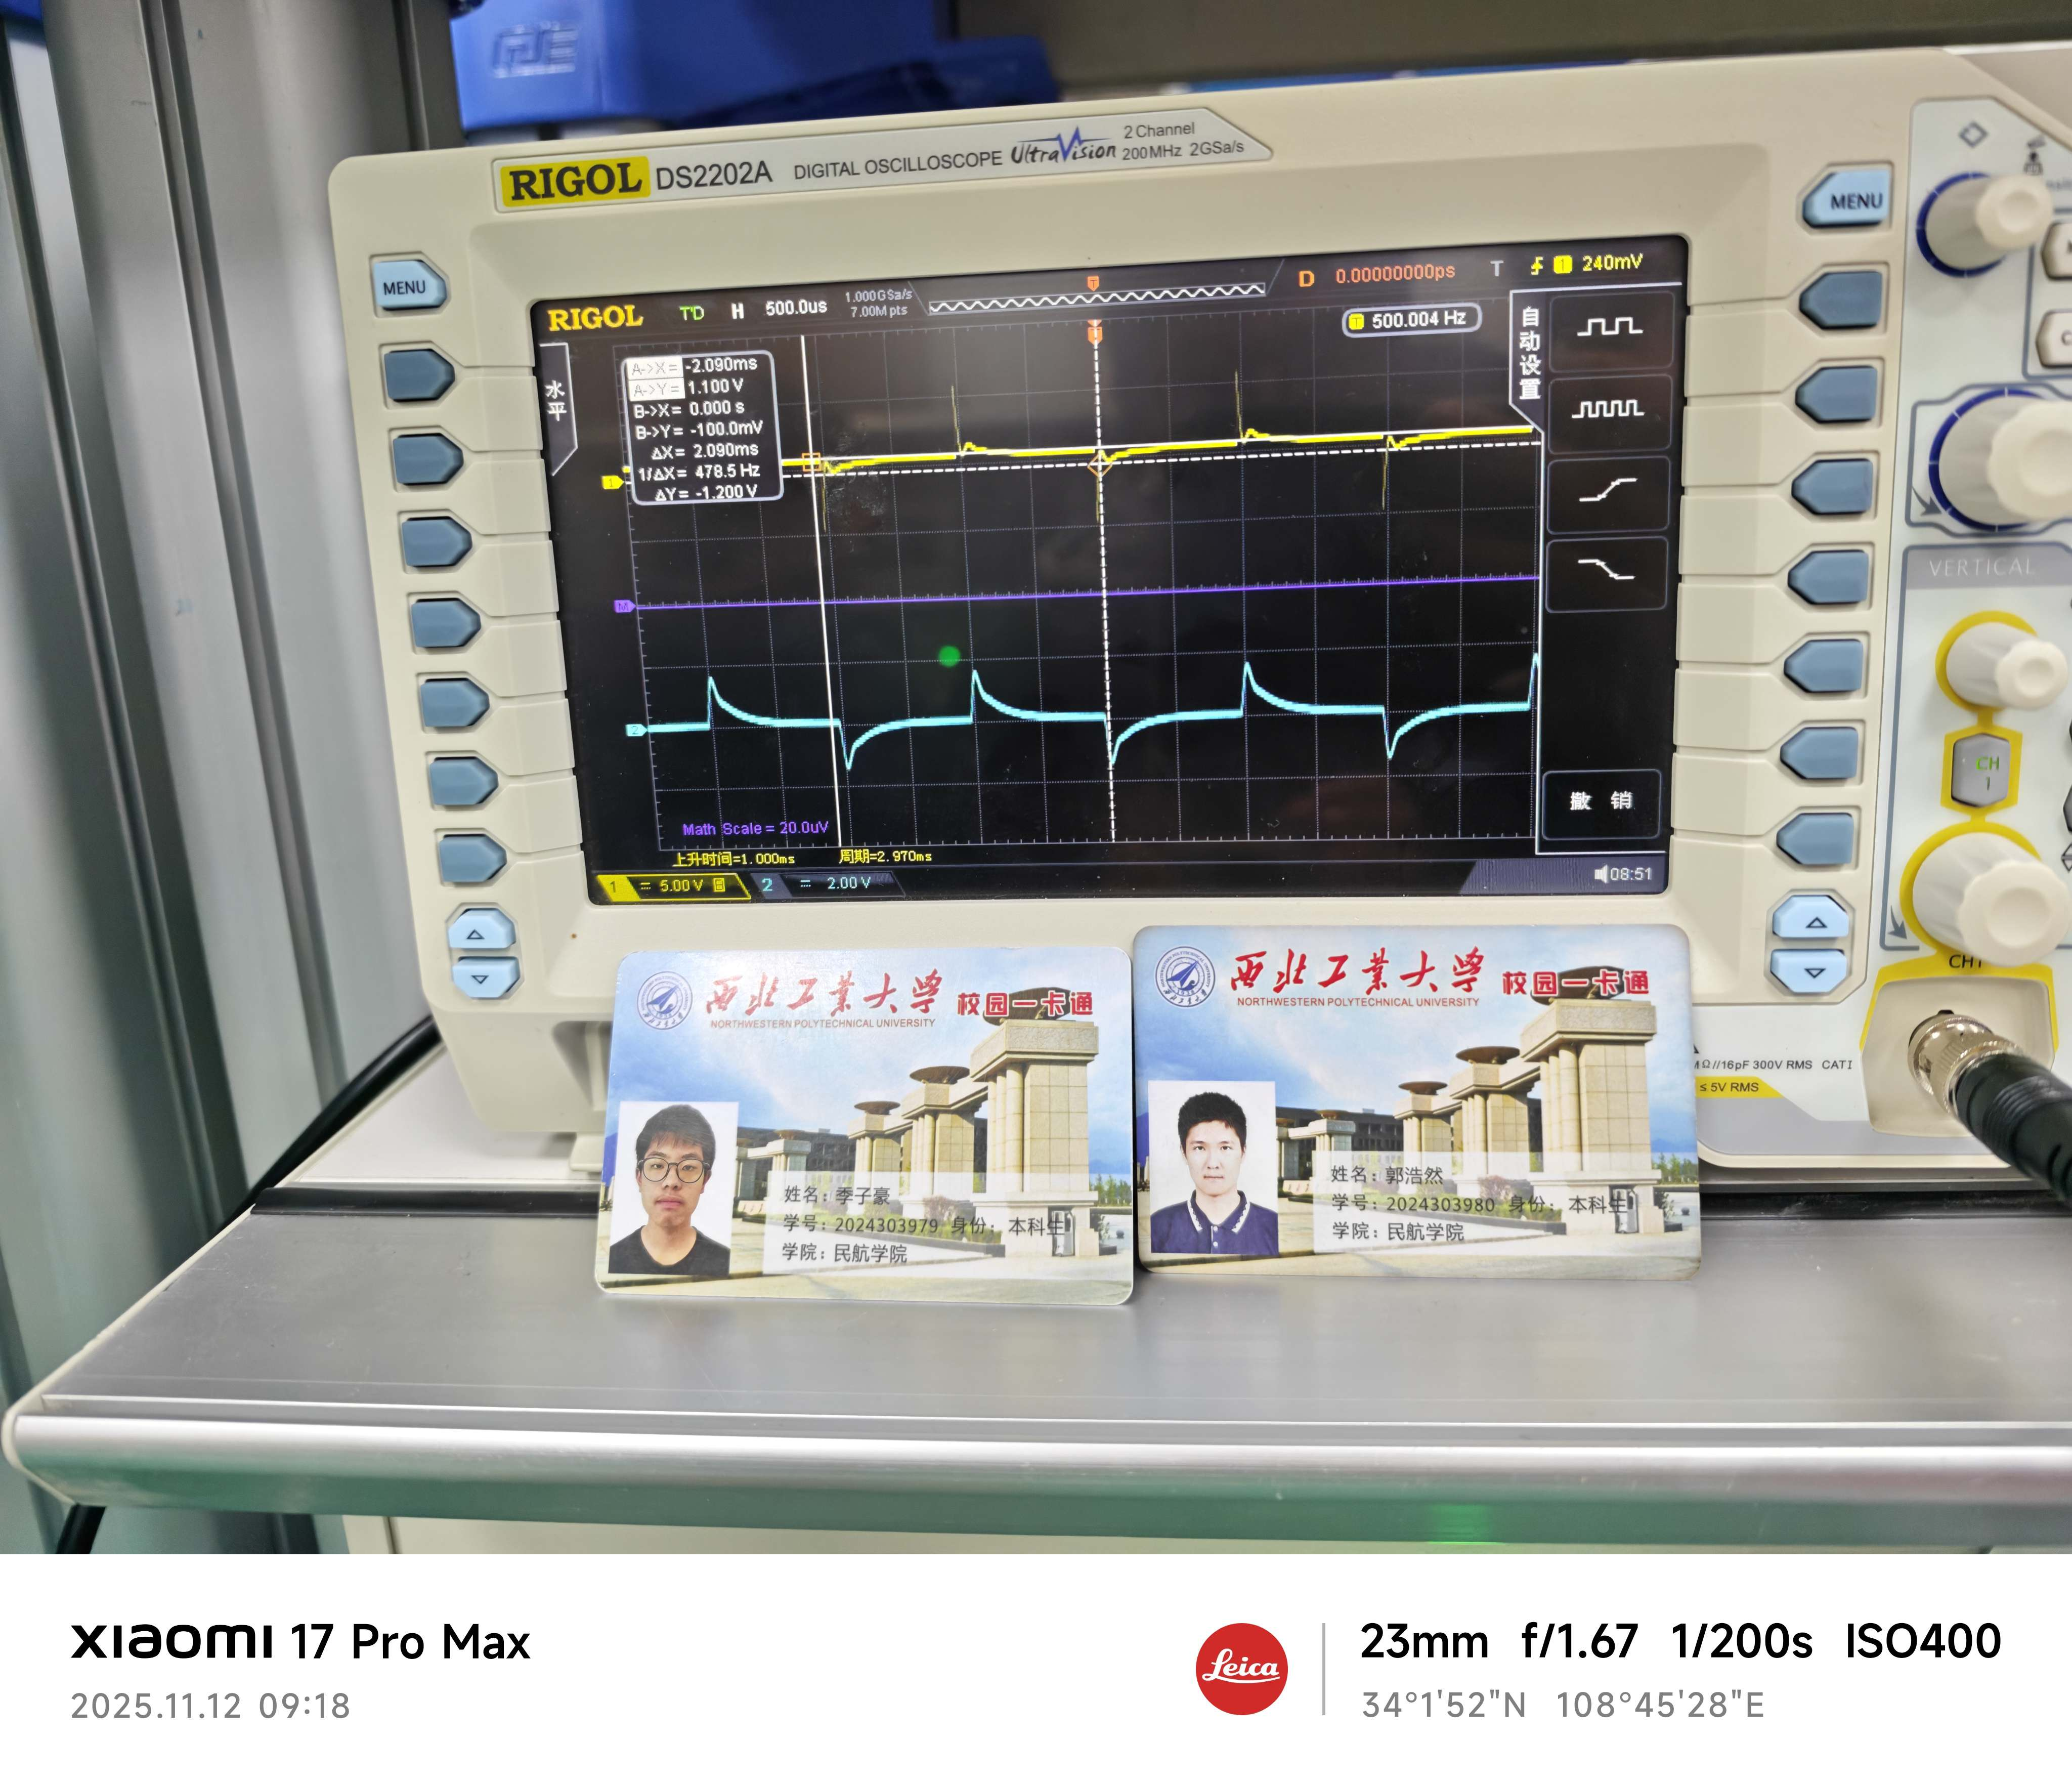
\includegraphics[width=\linewidth]{impulse_critical.jpg}
        \caption{临界阻尼状态}
        \label{fig:impulse_critical}
    \end{subfigure}
    \hfill
    \begin{subfigure}{0.32\textwidth}
        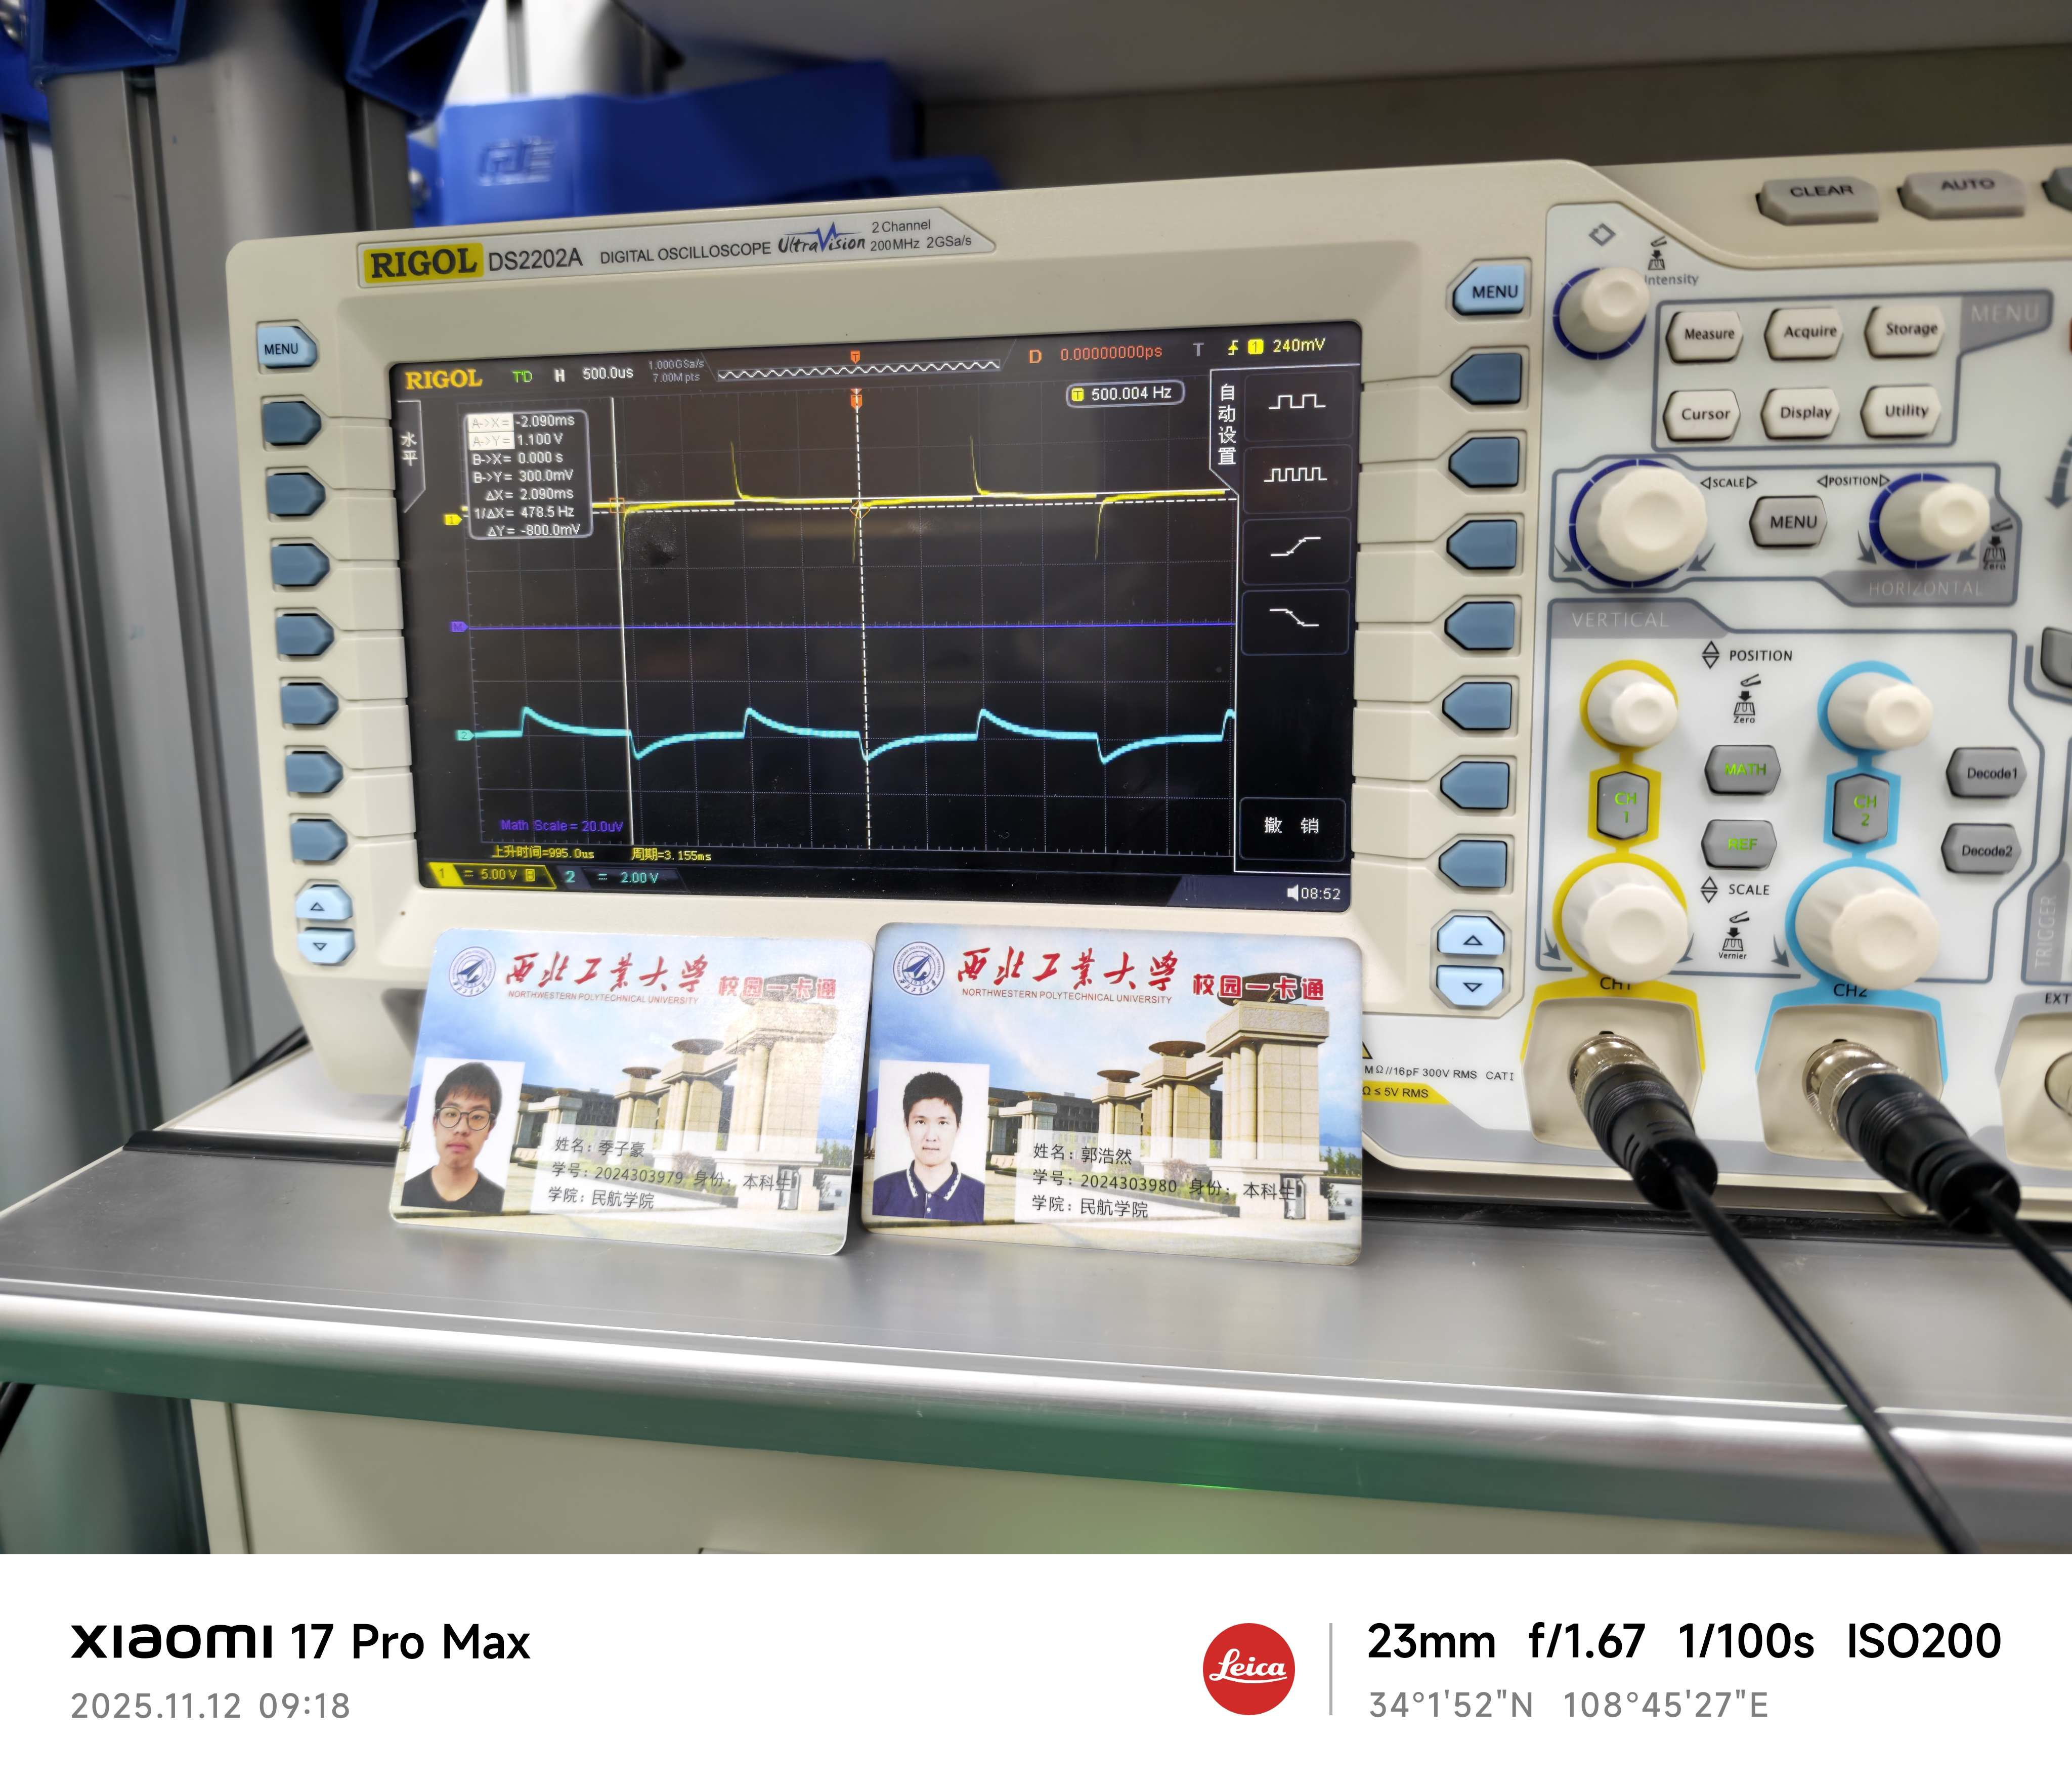
\includegraphics[width=\linewidth]{impulse_overdamped.jpg}
        \caption{过阻尼状态}
        \label{fig:impulse_over}
    \end{subfigure}
    \caption{冲激响应在不同阻尼状态下的示波器波形}
    \label{fig:impulse_waveforms}
\end{figure}


\subsection{参数测量数据}
在观察波形的同时，对各状态下的关键参数进行了测量，详细数据记录在表 \ref{tab:step_data} 和表 \ref{tab:impulse_data} 中。

% --- 阶跃响应数据表 (代码与之前相同) ---
\begin{table}[htbp]
    \centering
    \caption{阶跃响应参数测量数据}
    \label{tab:step_data}
    \renewcommand{\arraystretch}{1.5}
    \begin{tabular}{l c c c}
        \toprule
        \textbf{测量项目} & \textbf{欠阻尼状态} & \textbf{临界阻尼状态} & \textbf{过阻尼状态} \\
        \midrule
        电阻测量值 R & \SI{11.6}{\ohm} & \SI{484}{\ohm} & \SI{1109}{\ohm} \\
        \addlinespace
        TP12 激励波形 & \makecell{A = \SI{975}{\milli\volt} \\ T = \SI{2}{\milli\second} \\ $T_1$ = \SI{1}{\milli\second}} & \makecell{A = \SI{975}{\milli\volt} \\ T = \SI{2}{\milli\second} \\ $T_1$ = \SI{1}{\milli\second}} & \makecell{A = \SI{975}{\milli\volt} \\ T = \SI{2}{\milli\second} \\ $T_1$ = \SI{1}{\milli\second}} \\
        \addlinespace
        TP14 响应波形 & \makecell{A = \SI{969}{\milli\volt} \\ T = \SI{2}{\milli\second} \\ $T_1$ = \SI{1}{\milli\second} \\ $\tau$ = \SI{34}{\micro\second}} & \makecell{A = \SI{962}{\milli\volt} \\ T = \SI{2}{\milli\second} \\ $T_1$ = \SI{1}{\milli\second} \\ $\tau$ = \SI{70}{\micro\second}} & \makecell{A = \SI{940}{\milli\volt} \\ T = \SI{2}{\milli\second} \\ $T_1$ = \SI{1}{\milli\second} \\ $\tau$ = \SI{286}{\micro\second}} \\
        \bottomrule
    \end{tabular}
\end{table}

% --- 冲激响应数据表 (代码与之前相同) ---
\begin{table}[htbp]
    \centering
    \caption{冲激响应参数测量数据}
    \label{tab:impulse_data}
    \renewcommand{\arraystretch}{1.5}
    \begin{tabular}{l c c c}
        \toprule
        \textbf{测量项目} & \textbf{欠阻尼状态} & \textbf{临界阻尼状态} & \textbf{过阻尼状态} \\
        \midrule
        电阻测量值 R & \SI{3.0}{\ohm} & \SI{287}{\ohm} & \SI{1100}{\ohm} \\
        \addlinespace
        TP12 激励波形 & \makecell{A = \SI{1.988}{\volt} \\ T = \SI{2}{\milli\second} \\ $T_1$ = \SI{1}{\milli\second}} & \makecell{A = \SI{1.988}{\volt} \\ T = \SI{2}{\milli\second} \\ $T_1$ = \SI{1}{\milli\second}} & \makecell{A = \SI{1.988}{\volt} \\ T = \SI{2}{\milli\second} \\ $T_1$ = \SI{1}{\milli\second}} \\
        \addlinespace
        TP14 响应波形 & \makecell{A = \SI{820}{\milli\volt} \\ T = \SI{2}{\milli\second} \\ $T_1$ = \SI{1}{\milli\second} \\ $\tau$ = \SI{20}{\micro\second}} & \makecell{A = \SI{270}{\milli\volt} \\ T = \SI{2}{\milli\second} \\ $T_1$ = \SI{1}{\milli\second} \\ $\tau$ = \SI{90}{\micro\second}} & \makecell{A = \SI{220}{\milli\volt} \\ T = \SI{2}{\milli\second} \\ $T_1$ = \SI{1}{\milli\second} \\ $\tau$ = \SI{120}{\micro\second}} \\
        \bottomrule
    \end{tabular}
\end{table}


\subsection{综合分析}
结合图 \ref{fig:step_waveforms}、\ref{fig:impulse_waveforms} 所示的波形和表 \ref{tab:step_data}、\ref{tab:impulse_data} 的数据可以看出：
\begin{enumerate}
    \item \textbf{电阻与阻尼状态的关系：} 实验测得的电阻值 R 随着系统从欠阻尼、临界阻尼到过阻尼状态转变而显著增大。这与实验原理中 $R$ 与 $2\sqrt{L/C}$ 的大小关系完全吻合，验证了电阻是影响本 RLC 电路阻尼状态的关键参数。
    \item \textbf{阶跃响应分析：} 如图 \ref{fig:step_waveforms} 所示，在欠阻尼状态下，响应波形出现了明显的过冲和振荡；在临界阻尼状态下，波形最快达到稳定且无过冲；在过阻尼状态下，响应非常平缓，无过冲但上升时间最长。这与表 \ref{tab:step_data} 中响应时间常数 $\tau$ 从 \SI{34}{\micro\second} 增加到 \SI{286}{\micro\second} 的趋势一致。
    \item \textbf{冲激响应分析：} 如图 \ref{fig:impulse_waveforms} 所示，阻尼对冲激响应的峰值影响剧烈。随着阻尼增加，响应峰值迅速衰减，恢复到零的时间也相应变化。这说明阻尼越大，系统对瞬时冲击的能量耗散越快，抑制作用越强，与表 \ref{tab:impulse_data} 中峰值幅度从 \SI{820}{\milli\volt} 锐减至 \SI{220}{\milli\volt} 的数据相符。
\end{enumerate}
综上所述，实验波形和测量数据清晰地展示了二阶 RLC 电路在不同阻尼条件下对阶跃和冲激信号的响应特性，与理论预期高度一致。

\newpage

\section{信号的 Matlab 仿真与分析}

本章节展示了使用 Matlab 对一系列信号进行仿真和变换的结果。

\begin{figure}[H]
    \centering
    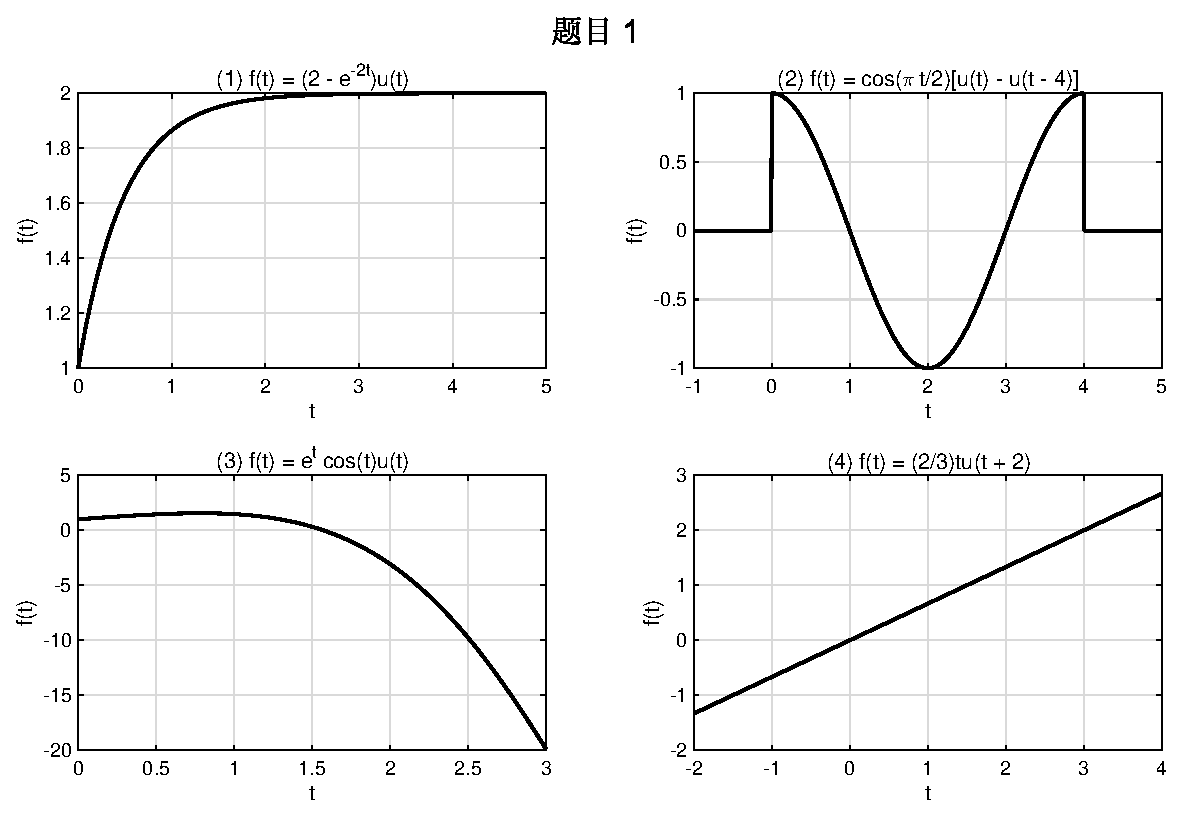
\includegraphics[width=0.7\textwidth]{T1.eps}
    \caption{题目 1：连续时间信号波形}
    \label{fig:T1}
\end{figure}

\begin{figure}[H]
    \centering
    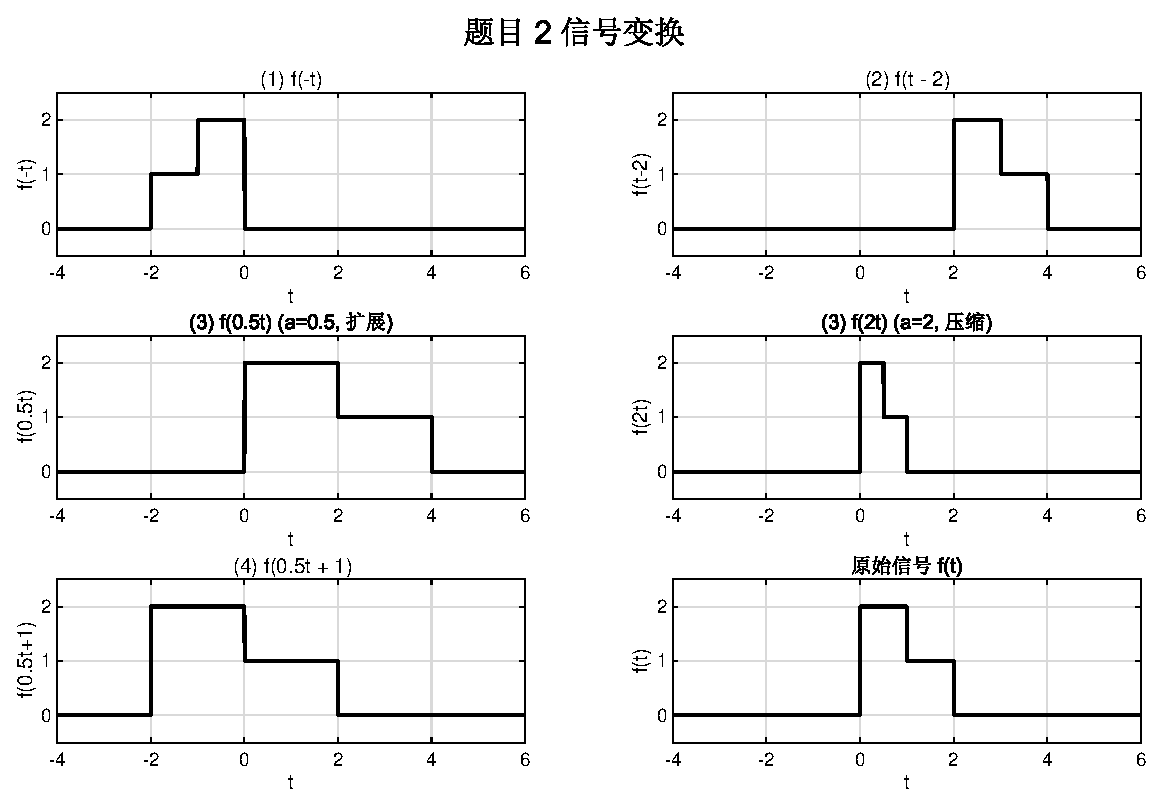
\includegraphics[width=0.8\textwidth]{T2.eps}
    \caption{题目 2：信号 f(t) 的基本变换}
    \label{fig:T2}
\end{figure}
\begin{figure}[H]
    \centering
    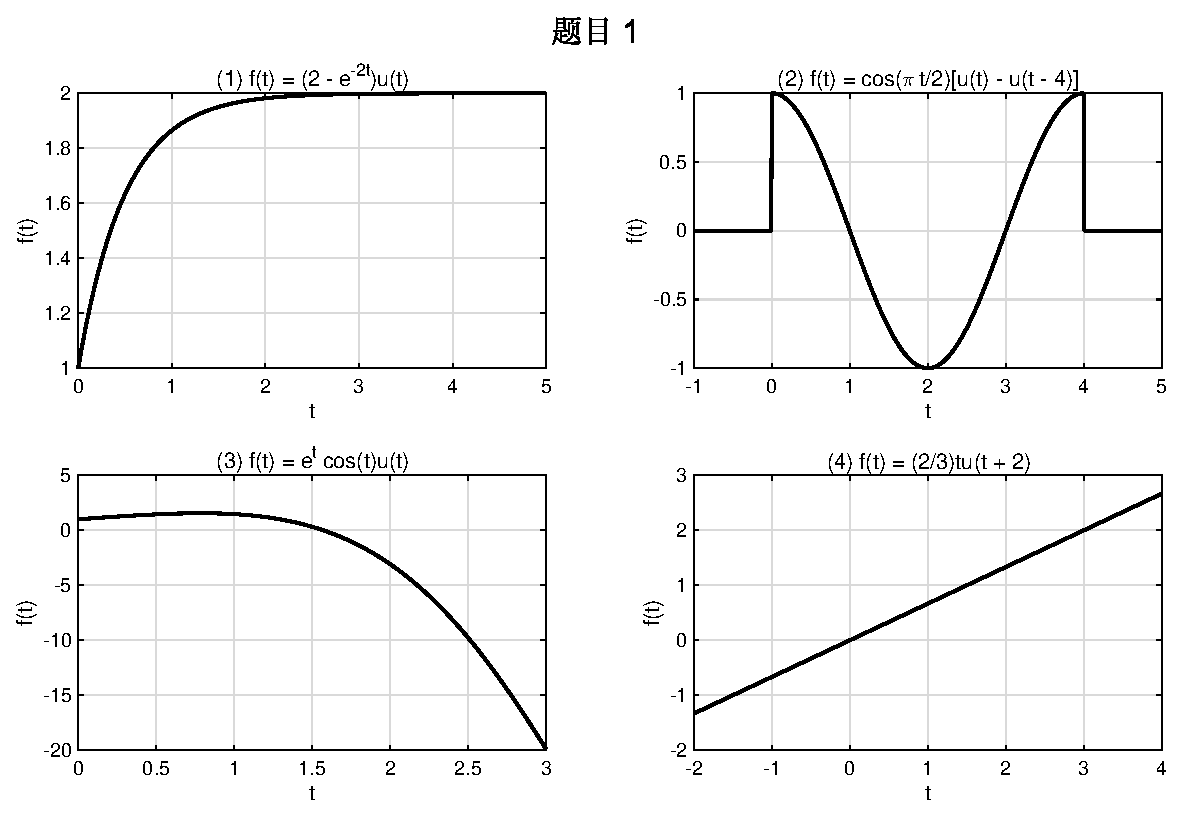
\includegraphics[width=0.8\textwidth]{T3.eps}
    \caption{题目 3：复信号 $f(t) = 2e^{j(t+\pi/4)}$ 的各分量}
    \label{fig:T3}
\end{figure}


\section{结论}
本次实验通过搭建 RLC 串联电路，成功观察并测量了二阶系统在不同阻尼条件下的阶跃响应与冲激响应，得出以下结论：

\begin{enumerate}
    \item \textbf{验证了阻尼理论：} 实验结果清晰地表明，电路的阻尼状态由电阻 R 的值决定。通过改变 R 值，可以使电路呈现出欠阻尼、临界阻尼和过阻尼三种不同的响应特性，这与 $R$ 和 $2\sqrt{L/C}$ 的理论关系完全一致。

    \item \textbf{掌握了响应特性：}
    \begin{itemize}
        \item \textbf{阶跃响应：} 欠阻尼状态响应速度快但伴有超调和振荡；临界阻尼状态响应速度最快且无超调，是理想的快速响应状态；过阻尼状态响应平稳无超调，但响应时间最长。
        \item \textbf{冲激响应：} 阻尼越大，系统对瞬时冲击的抑制能力越强，响应峰值越低，能量耗散越快。
    \end{itemize}

    \item \textbf{探究了响应关系：} 实验中通过将方波（近似阶跃信号）输入微分电路来获得冲激响应波形，直观地验证了冲激响应是阶跃响应的微分这一基本理论关系。

    \item \textbf{提升了测量技能：} 通过本次实验，熟练掌握了使用示波器观察动态波形、测量上升时间、峰值等动态性能指标的方法，并对二阶系统的时域分析有了更深刻的物理认识。
\end{enumerate}

综上所述，本实验成功达成了预定的实验目的，加深了对二阶系统动态特性的理解。

\end{document}